\documentclass[12pt,a4paper,oneside]{report}
\usepackage[a4paper,margin=1in]{geometry}
\usepackage{mathptmx}            % Times New Roman text and maths
\usepackage[T1]{fontenc}
\usepackage[utf8]{inputenc}
\usepackage{graphicx,float,array,booktabs,enumitem,amsmath,amssymb,xcolor}
\usepackage{caption}
\usepackage{listings}
\usepackage{setspace}
\setlength{\textfloatsep}{10pt plus 2pt minus 2pt}
\setlength{\intextsep}{10pt plus 2pt minus 2pt}
\setlength{\floatsep}{10pt plus 2pt minus 2pt}
\renewcommand{\topfraction}{0.9}\renewcommand{\bottomfraction}{0.8}
\renewcommand{\textfraction}{0.08}\renewcommand{\floatpagefraction}{0.75}
\usepackage{titlesec}
\usepackage[hidelinks]{hyperref}
\setstretch{1.0}
\setlength{\parskip}{4pt}
\setlength{\parindent}{0pt}
\captionsetup{font={small},labelfont={bf},justification=centering,skip=4pt}
\titleformat{\chapter}[hang]{\normalfont\fontsize{14}{16}\bfseries}{\chaptertitlename\ \thechapter:}{0.5em}{}
\titlespacing*{\chapter}{0pt}{0pt}{10pt}
\titleformat{\section}{\normalfont\fontsize{14}{16}\bfseries}{\thesection}{0.6em}{}
\titleformat{\subsection}{\normalfont\fontsize{12}{14}\bfseries}{\thesubsection}{0.6em}{}
\renewcommand{\listfigurename}{List of Figures}
\lstset{basicstyle=\ttfamily\scriptsize,breaklines=true,frame=single,columns=fullflexible,
  captionpos=b,showstringspaces=false,tabsize=4,language=Python,
  commentstyle=\color{black!60},keywordstyle=\bfseries,breakatwhitespace=false}
\pagestyle{plain}
\begin{document}
\pagenumbering{roman}
% ---------------- cover ----------------
\begin{titlepage}
\centering
{\fontsize{14}{16}\bfseries Department of Computer Engineering\par}
\vspace{4pt}
{\fontsize{14}{16}\bfseries St. Francis Institute of Technology\par}
\vspace{4pt}
{\fontsize{14}{16}\bfseries University of Mumbai\par}
\vspace{4pt}
{\fontsize{14}{16}\bfseries 2026-2027\par}
\vspace{1.4cm}
{\fontsize{14}{16}\bfseries A Mini Project Report On\par}
\vspace{1cm}
{\fontsize{14}{16}\bfseries ``Prediction of Heart Disease using Ensemble Learning: A Reproducible Re-implementation and Extension of the MPBE Model''\par}
\vspace{1.2cm}
{\fontsize{14}{16}\bfseries Subject: Machine Learning [CSL 701]\par}
\vspace{1cm}

\includegraphics[width=3.4cm]{figures/sfit_logo.png}\par
\vspace{1cm}
{\fontsize{14}{16}\bfseries Under the guidance of\par}
\vspace{4pt}
{\fontsize{14}{16}\bfseries Dr. Nazneen Ansari\par}
\vspace{1cm}
{\fontsize{14}{16}\bfseries By\par}
\vspace{4pt}
{\fontsize{14}{16}\bfseries Salil Mahale (Roll no. 53, PID no. 232085)\par}
{\fontsize{14}{16}\bfseries BE CMPN B, Batch 3\par}
\vfill
\end{titlepage}
\clearpage
\chapter*{Abstract}
\addcontentsline{toc}{chapter}{Abstract}
Cardiovascular disease remains the leading cause of death worldwide, and inexpensive clinical attributes such as age, chest pain type, resting blood pressure and exercise test results are routinely available long before an angiogram is ordered. This mini project re-implements the \textbf{MPBE} model (MinMax normalized Pearson coefficient Bagging Ensemble) proposed by Muthulakshmi et al. [1] and extends it in three directions. First, the model is evaluated not only on the \textbf{UCI Cleveland} dataset (303 patients) used in the original work but also on a \textbf{combined five source dataset} (Cleveland, Hungarian, Switzerland, Long Beach VA and Statlog, 918 unique patients) to test generalisation. Second, the bagging ensemble is compared against \textbf{Voting, Stacking, AdaBoost, Gradient Boosting and XGBoost} as well as six single classifiers. Third, evaluation uses \textbf{stratified 10-fold cross validation} with scaling fitted inside each fold, and reports accuracy, precision, recall, F1 score and ROC-AUC rather than accuracy alone. On Cleveland, MPBE reaches 82.46\% cross validated accuracy (ROC-AUC 0.912) and 86.89\% on a 20\% hold-out split; the 95.33\% reported in the original paper could not be reproduced under a leakage free protocol. On the combined dataset, MPBE is the best of all fourteen models with 80.84\% accuracy and ROC-AUC 0.884. The project concludes that heterogeneous bagging is a robust choice for tabular clinical data, that ensemble gains over strong single learners are modest, and that honest cross validated reporting matters more than a headline accuracy.
\vspace{1.5em}
\par\vspace{0.5em}
{\small\setlength{\parskip}{0pt}\let\clearpage\relax\par\tableofcontents}
\clearpage
\listoffigures
\addcontentsline{toc}{chapter}{List of Figures}
\par\vspace{1.2em}\par
{\let\clearpage\relax \listoftables}
\addcontentsline{toc}{chapter}{List of Tables}
\par\vspace{1.4em}
\noindent{\fontsize{14}{16}\bfseries List of Abbreviations}\par\vspace{0.6em}
\addcontentsline{toc}{chapter}{List of Abbreviations}
\begin{tabular}{ll}
\textbf{AUC} & Area Under the ROC Curve \\
\textbf{CART} & Classification and Regression Tree \\
\textbf{CV} & Cross Validation \\
\textbf{DT} & Decision Tree \\
\textbf{EDA} & Exploratory Data Analysis \\
\textbf{GB} & Gradient Boosting \\
\textbf{KNN} & K-Nearest Neighbours \\
\textbf{LR} & Logistic Regression \\
\textbf{ML} & Machine Learning \\
\textbf{MPBE} & MinMax normalized Pearson coefficient Bagging Ensemble \\
\textbf{NB} & Naive Bayes \\
\textbf{RBF} & Radial Basis Function \\
\textbf{RF} & Random Forest \\
\textbf{ROC} & Receiver Operating Characteristic \\
\textbf{SVM} & Support Vector Machine \\
\textbf{UCI} & University of California, Irvine (ML Repository) \\
\textbf{XGBoost} & Extreme Gradient Boosting \\
\end{tabular}

\clearpage
\pagenumbering{arabic}
\chapter{Introduction}
\section{Introduction}
\textbf{Heart disease} is the single largest cause of mortality in India and globally. Roughly one in four heart related deaths in India occurs in people younger than forty, which makes \textbf{early prediction} from routinely collected clinical measurements a genuinely valuable problem [1]. The measurements involved (age, sex, chest pain type, resting blood pressure, cholesterol, fasting blood sugar, resting ECG, maximum heart rate, exercise induced angina, ST depression, ST slope, number of vessels seen on fluoroscopy and thalassemia status) are cheap, non-invasive or already part of a standard cardiac work-up, so a model that predicts the presence of disease from them can act as a screening aid before expensive angiography.

\textbf{Machine learning} offers a family of classifiers that learn the mapping from these attributes to a diagnosis. No single classifier is best on every dataset, and individual models such as a decision tree are unstable: small changes in the training data produce very different trees. \textbf{Ensemble learning} addresses this by training several models and combining their decisions. \textbf{Bagging} (bootstrap aggregating) trains each member on a bootstrap resample of the training set and averages their votes, which reduces variance; \textbf{boosting} trains members sequentially, each focusing on the mistakes of the previous ones, which reduces bias; \textbf{stacking} learns how to weight the members with a second level model.

Muthulakshmi, Parveen and Rajeswari [1] proposed the \textbf{MPBE} model, a bagging ensemble whose base learners are a Decision Tree, a Random Forest, a Naive Bayes classifier and a Support Vector Machine, trained on Pearson correlation selected and MinMax normalised features of the UCI Cleveland dataset, and reported 95.33\% accuracy. This project takes that paper as its starting point, re-implements the method from the description given, and asks two questions the original paper does not answer: does the result hold under a strict cross validated protocol, and does it hold on a larger, more heterogeneous population?

\section{Problem Definition}
Given a patient record of thirteen clinical attributes, predict the \textbf{binary label} target = 1 (presence of heart disease, i.e. more than 50\% narrowing of a major vessel) or target = 0 (absence). The specific objectives of this project are:

\begin{enumerate}
  \item Re-implement the MPBE pipeline of [1] (MinMax scaling, Pearson correlation feature selection, four bagging ensembles of 100 estimators each, mean aggregation) in Python with scikit-learn.
  \item Evaluate it on the UCI Cleveland dataset (303 records) and on a combined dataset built from all five UCI heart disease sources (918 unique records after de-duplication).
  \item Compare MPBE with six single classifiers (DT, RF, NB, SVM, LR, KNN) and six alternative ensembles (homogeneous Bagging, soft Voting, hard Voting, Stacking, AdaBoost, Gradient Boosting, XGBoost).
  \item Use stratified 10-fold cross validation and an 80:20 stratified hold-out, reporting accuracy, precision, recall, F1 score, ROC-AUC and confusion matrices.
  \item Quantify the contribution of the Pearson feature selection step through an ablation run on all 13 attributes.
  \item Provide a small desktop interface that loads the trained model and predicts for a single patient.
\end{enumerate}

\section{Prerequisites}
The reader is assumed to know the basics of \textbf{supervised classification}, the train and test split, the confusion matrix and its derived metrics, and to have seen decision trees, Naive Bayes, SVM and logistic regression. The relevant ensemble concepts (bagging, boosting, stacking, voting) are summarised in chapter 3. The implementation requires Python 3.10 or later with scikit-learn, xgboost, pandas, numpy, matplotlib and seaborn; the exact versions are listed in chapter 5.

\chapter{Literature Review}
Twenty research papers on heart disease prediction with machine learning were reviewed, with an emphasis on \textbf{ensemble methods}, \textbf{feature selection} and \textbf{evaluation protocol}, since those are the three ingredients of the MPBE model. Six of them are the papers the base paper itself builds on [2]-[7]; the remaining fourteen are later or more widely cited works that give a fuller picture of what is achievable on the same data [8]-[21]. Table 2.1 records the dataset, technique and headline result of each. Longer summaries of every paper, together with its relevance to this project, are provided in the companion document ML\_MiniProject\_Literature\_Review.docx.

\begin{table}[htbp]
\centering
\caption{The twenty reviewed papers}
\footnotesize
\begin{tabular}{>{\raggedright\arraybackslash}p{0.057\textwidth}>{\raggedright\arraybackslash}p{0.057\textwidth}>{\raggedright\arraybackslash}p{0.193\textwidth}>{\raggedright\arraybackslash}p{0.385\textwidth}>{\raggedright\arraybackslash}p{0.249\textwidth}}
\hline
\textbf{Ref} & \textbf{Year} & \textbf{Dataset} & \textbf{Technique} & \textbf{Reported result} \\
\hline
{}[2] & 2022 & Cleveland (UCI) & Multilayer Perceptron and K-Nearest Neighbour & MLP 82.47\% accuracy, AUC 86.41\% \\
{}[3] & 2022 & Cleveland (UCI) & Random Forest, KNN, Decision Tree, XGBoost plus a stacked ensemble and K-modes clustering & Stacked model reported 88.7\% accuracy \\
{}[4] & 2020 & Cleveland and Framingham & Homogeneous ensemble of CART trees combined by an accuracy based weighted aging classifier & 93\% on Cleveland, 91\% on Framingham \\
{}[5] & 2018 & Cleveland (UCI) & Seven classifiers (LR, KNN, ANN, SVM, NB, DT, RF) with Relief, mRMR and LASSO feature selection under 10-fold CV & Logistic Regression with Relief features 89\% accuracy \\
{}[6] & 2022 & Cleveland, Statlog and a Mendeley cardiovascular dataset & Majority voting and stacking ensembles with GridSearch tuned base learners & Up to 96\% accuracy on the combined data \\
{}[7] & 2020 & Cleveland (UCI) & Correlation based feature selection followed by an ensemble of Random Forest, SVM and Naive Bayes & Ensemble 86.8\% accuracy versus 82 to 84\% for the base learners \\
{}[8] & 2019 & Cleveland (UCI) & Hybrid Random Forest with a Linear Model over selected feature combinations & 88.7\% accuracy \\
{}[9] & 2019 & Cleveland (UCI) & Bagging, boosting, stacking and majority voting over NB, C4.5, MLP, PART and RF, with and without feature selection & Majority vote improved weak classifiers by up to 7.26\% \\
{}[10] & 2021 & Cleveland (UCI) & Bagging, boosting and stacking compared with tuned single models & Stacked ensemble of KNN, RF and SVM best at about 75\% accuracy \\
{}[11] & 2021 & Kaggle heart dataset & KNN, DT and RF with feature importance analysis & RF reported 100\% on a leaky Kaggle copy of the data \\
{}[12] & 2020 & Cleveland (UCI) & Naive Bayes, Decision Tree, KNN and Random Forest & KNN best at 90.8\% accuracy on one split \\
{}[13] & 2021 & Cleveland (UCI) & Isolation Forest outlier removal, LASSO feature selection, classical ML and a deep neural network & Deep learning 94.2\% accuracy \\
{}[14] & 2021 & Cleveland (UCI) & Bagging, AdaBoost, Gradient Boosting, Random Forest and stacking & Ensembles outperformed single learners; boosting and stacking strongest \\
{}[15] & 2020 & Cleveland (UCI) & Feature selection (Relief, mRMR, LASSO and a proposed FCMIM) with SVM, LR, ANN, KNN, DT and NB & SVM with FCMIM selected features 92.37\% accuracy \\
{}[16] & 2024 & Cleveland and Framingham & Random Forest, AdaBoost and XGBoost tuned with Bayesian optimization, explained with SHAP & XGBoost 97.1\% on Cleveland, 92.1\% on Framingham \\
{}[17] & 2023 & Three merged Kaggle heart datasets & Extra Trees, RF, XGBoost and CatBoost with GridSearchCV & Extra Trees 98.15\% accuracy on an 80:20 split \\
{}[18] & 2023 & Cleveland and IEEE Dataport & RF, KNN, LR, NB, Gradient Boosting, AdaBoost and a soft voting ensemble tuned with GridSearchCV & Soft voting 95\% on IEEE Dataport, LR 90.16\% on Cleveland \\
{}[19] & 2022 & Cleveland, Statlog and a Kaggle heart dataset & SVM, KNN, DT, RF, LR, NB and boosting with and without grid search & Tuned RF and SVM close to 99\% on some splits \\
{}[20] & 2024 & Heart patient dataset & Stacked ensemble whose hyperparameters are chosen by Grey Wolf Optimization & Reported improvement over unoptimized stacking \\
{}[21] & 2025 & Framingham and other heart datasets & Soft voting of XGBoost and Explainable Boosting Machine with nested CV, SHAP and LIME & Reports calibrated, leakage controlled results with confidence intervals \\
\hline
\end{tabular}
\end{table}

\section{Themes in the Reviewed Literature}
\subsection{Ensemble Design}
Latha and Jeeva [9] quantified the gain of each ensemble family over weak base classifiers on Cleveland: majority voting lifted accuracy by up to 7.26 points, bagging by 6.92 and boosting by 5.94. Karadeniz et al. [14] compared the same families under one preprocessing pipeline and found boosting and stacking marginally ahead. Mienye et al. [4] showed that the \textbf{aggregation rule} matters as much as the members: an accuracy weighted, aging combination of CART models reached 93\% on Cleveland where plain voting did not. Alim et al. [7] and Alqahtani et al. [3] both built heterogeneous ensembles (RF, SVM, NB and tree based learners respectively) and reported 86.8\% and 88.7\%. The consistent message is that combining \textbf{different learner families} helps more than enlarging one family, which is precisely the design of MPBE, but that the gain over an already strong single learner is small.

\subsection{Feature Selection}
Haq et al. [5] compared Relief, mRMR and LASSO selectors across seven classifiers and found Logistic Regression on Relief selected features best at 89\%. Li et al. [15] proposed a conditional mutual information selector and reached 92.37\% with a linear SVM. Mohan et al. [8] searched over feature subsets to build the widely cited HRFLM hybrid at 88.7\%. Across these studies the attributes dropped are almost always \textbf{cholesterol and fasting blood sugar}, the two with the weakest correlation to the diagnosis, and the accuracy change is within one or two points. Our Pearson filter reaches the same conclusion by a simpler route.

\subsection{Evaluation Protocol and Reproducibility}
The widest spread in the literature comes from protocol rather than algorithm. Ali et al. [11] reported 100\% accuracy for Random Forest on a Kaggle copy of the data later shown to contain duplicate rows, so test patients also appeared in training. Ahmad et al. [19] ran every model twice, with and without GridSearchCV, and pushed several to near 99\% on single splits. Shorewala [10], by contrast, used a careful protocol and reported only about 75\% for the best stacked ensemble. Adekoya et al. [21] and Mienye and Jere [16] argue explicitly for nested cross validation, leakage control, calibration and SHAP based explanation as the criteria that decide clinical usefulness. This is the direction our evaluation follows.

\subsection{Datasets and Generalisation}
Doppala et al. [6] evaluated ensembles on Cleveland, Statlog and a Mendeley cardiovascular dataset and argued that a reliable model must agree across datasets. Asif et al. [17] merged three Kaggle datasets with common attributes before tuning, reaching 98.15\% on an 80:20 split. Bharti et al. [13] showed that outlier removal and normalisation move results by several points on their own. Pal et al. [2], Shah et al. [12] and Chandrasekhar and Peddakrishna [18] provide the single dataset baselines, in the 82\% to 90\% range, against which our Cleveland numbers can be read. Narasimhan and Victor [20] represent the current direction of metaheuristic optimizers wrapped around a stacked ensemble.

\section{Observations from the Review}
\begin{itemize}
  \item Almost every paper uses the 13 attribute UCI Cleveland data [22]; accuracies reported on it range from about 75\% to above 97\%, and the spread is explained mostly by protocol (single split versus cross validation, tuning, duplicate rows) rather than by the algorithm.
  \item Heterogeneous ensembles (bagging, stacking, soft voting) consistently outperform a single Decision Tree by 8 to 12 points but beat a well regularised single learner such as Logistic Regression or Naive Bayes by only 0 to 3 points [9], [14], [18].
  \item Feature selection helps slightly and mainly removes chol and fbs, which have the weakest correlation with the label [5], [7], [15].
  \item Recent work stresses leakage control, calibration and explainability over headline accuracy [16], [21]; this project follows that direction.
\end{itemize}

\chapter{Proposed Work / Methodology}
\section{System Architecture}
The system is a \textbf{sequential pipeline} with six stages: data loading, preprocessing (missing value imputation), Pearson correlation feature selection, MinMax scaling, ensemble training and evaluation. Scaling is placed inside a scikit-learn Pipeline so that it is fitted only on the training fold of each cross validation split; this is the one point where our design deliberately differs from the description in [1], which scales the whole dataset before splitting.

\begin{figure}[htbp]
\centering
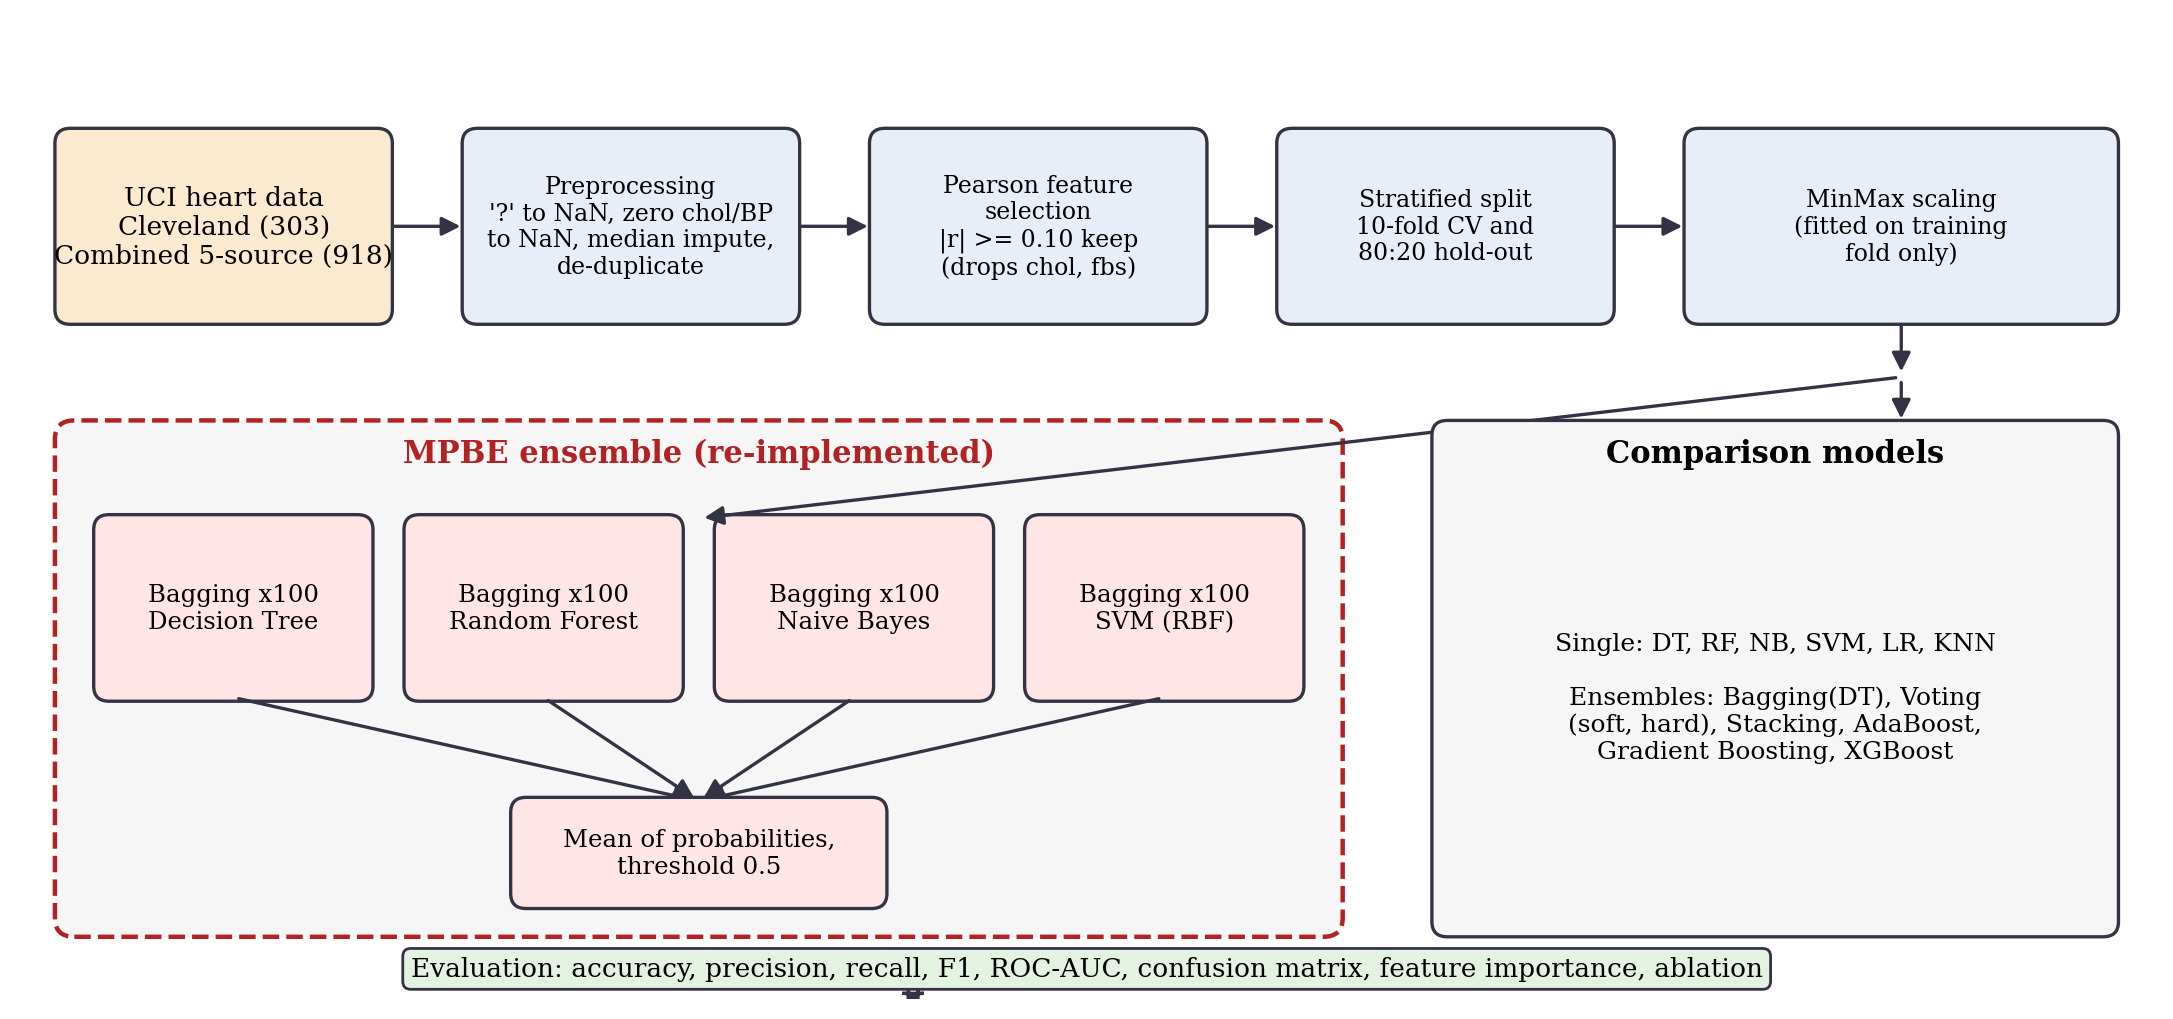
\includegraphics[width=0.88\textwidth]{figures/architecture.png}
\caption{Architecture of the proposed system (our re-implementation of MPBE with the added comparison branch)}
\end{figure}

\subsection{Description and Source of the Datasets}
\textbf{Dataset 1, Cleveland.} The processed Cleveland file from the UCI Machine Learning Repository [22] contains 303 patient records and 14 attributes (13 predictors and the diagnosis num in the range 0 to 4). Following [1] and nearly all prior work, num is binarised to target = 1 if num \textgreater{} 0. The class balance is 164 negatives and 139 positives. Six cells are missing (four in ca, two in thal).

\textbf{Dataset 2, Combined.} To test generalisation we concatenated all five UCI heart disease sources: Cleveland (303), Hungarian (294), Switzerland (123), Long Beach VA (200) [22] and Statlog (270) [23]. Statlog codes the label as 1 or 2 and was remapped to 0 or 1. The Hungarian, Swiss and VA records were collected with less complete protocols, so several attributes are missing; a cholesterol or blood pressure of 0 is physiologically impossible and was treated as missing. After removing exact duplicate rows the dataset holds 918 unique patients (508 positive, 410 negative). Duplicate removal matters because Statlog overlaps with Cleveland; leaving duplicates in would let test patients appear in training folds [11].

\begin{table}[htbp]
\centering
\caption{Attributes of the heart disease datasets}
\footnotesize
\begin{tabular}{>{\raggedright\arraybackslash}p{0.146\textwidth}>{\raggedright\arraybackslash}p{0.627\textwidth}>{\raggedright\arraybackslash}p{0.167\textwidth}}
\hline
\textbf{Attribute} & \textbf{Meaning} & \textbf{Type} \\
\hline
age & Age in years & Numeric \\
sex & Sex (1 = male, 0 = female) & Binary \\
cp & Chest pain type (1 typical angina, 2 atypical, 3 non-anginal, 4 asymptomatic) & Categorical \\
trestbps & Resting blood pressure in mm Hg & Numeric \\
chol & Serum cholesterol in mg/dl & Numeric \\
fbs & Fasting blood sugar greater than 120 mg/dl (1 = true) & Binary \\
restecg & Resting ECG result (0 normal, 1 ST-T abnormality, 2 LV hypertrophy) & Categorical \\
thalach & Maximum heart rate achieved & Numeric \\
exang & Exercise induced angina (1 = yes) & Binary \\
oldpeak & ST depression induced by exercise relative to rest & Numeric \\
slope & Slope of the peak exercise ST segment (1 up, 2 flat, 3 down) & Categorical \\
ca & Number of major vessels coloured by fluoroscopy (0 to 3) & Numeric \\
thal & Thalassemia (3 normal, 6 fixed defect, 7 reversible defect) & Categorical \\
target & 1 = presence of heart disease (num \textgreater{} 0), 0 = absence & Binary (label) \\
\hline
\end{tabular}
\end{table}

\subsection{Data Loading and Exploration}
Both datasets are read with pandas, the '?' marker is mapped to NaN, and missing values are filled with the \textbf{column median} computed on the whole dataset (this is the only preprocessing not done inside the CV fold; medians of a few cells cannot leak the label). Figures 3.2 to 3.4 summarise the exploratory analysis. The classes are roughly balanced in both datasets, so accuracy is a meaningful metric and no resampling is required. The age distribution shows the expected shift: patients with disease are older on average.

\begin{figure}[htbp]
\centering
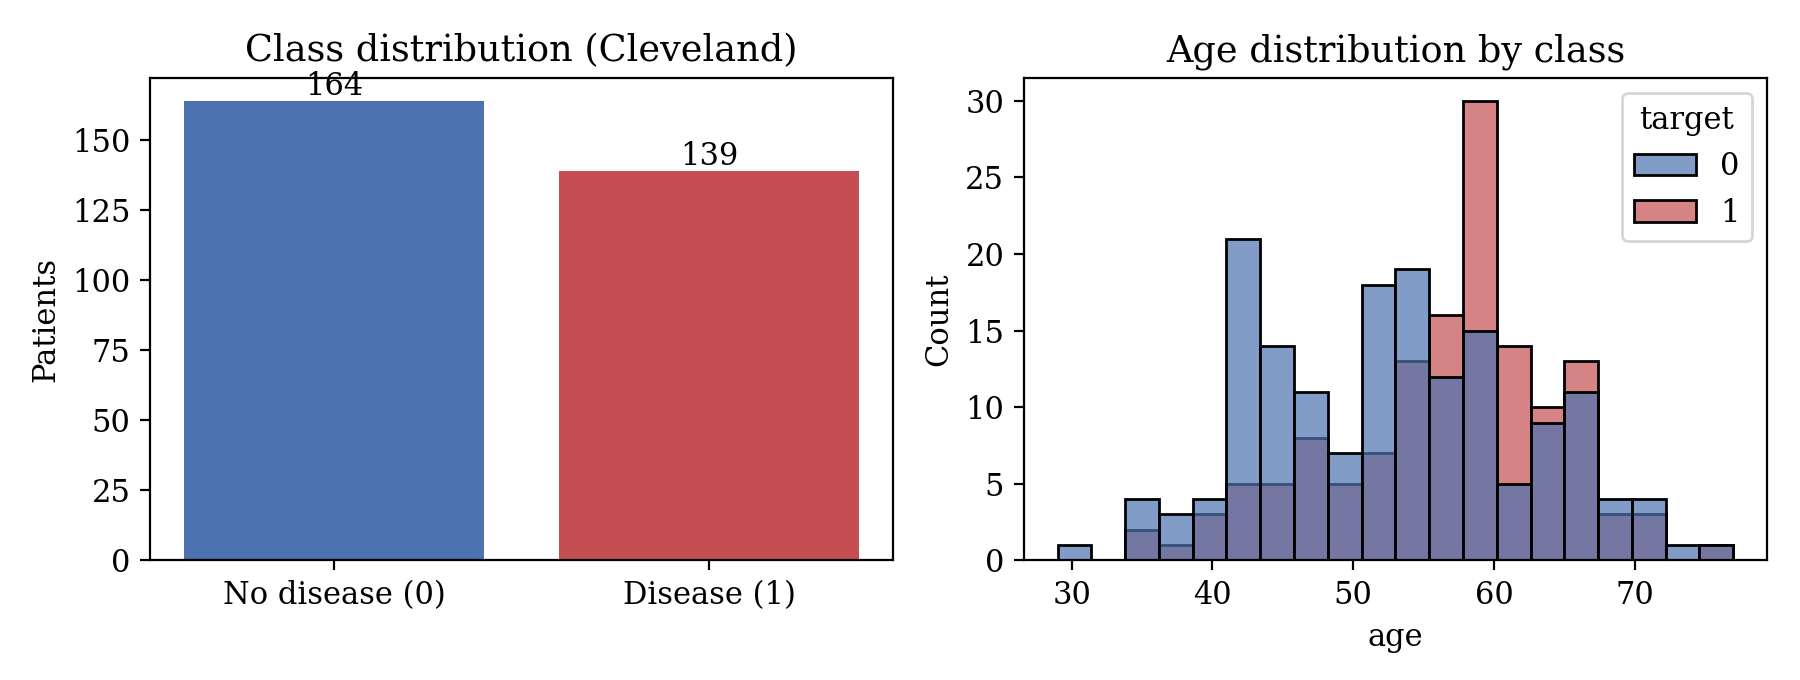
\includegraphics[width=0.62\textwidth]{figures/eda_cleveland.png}
\caption{Class balance and age distribution, Cleveland}
\end{figure}

\begin{figure}[htbp]
\centering
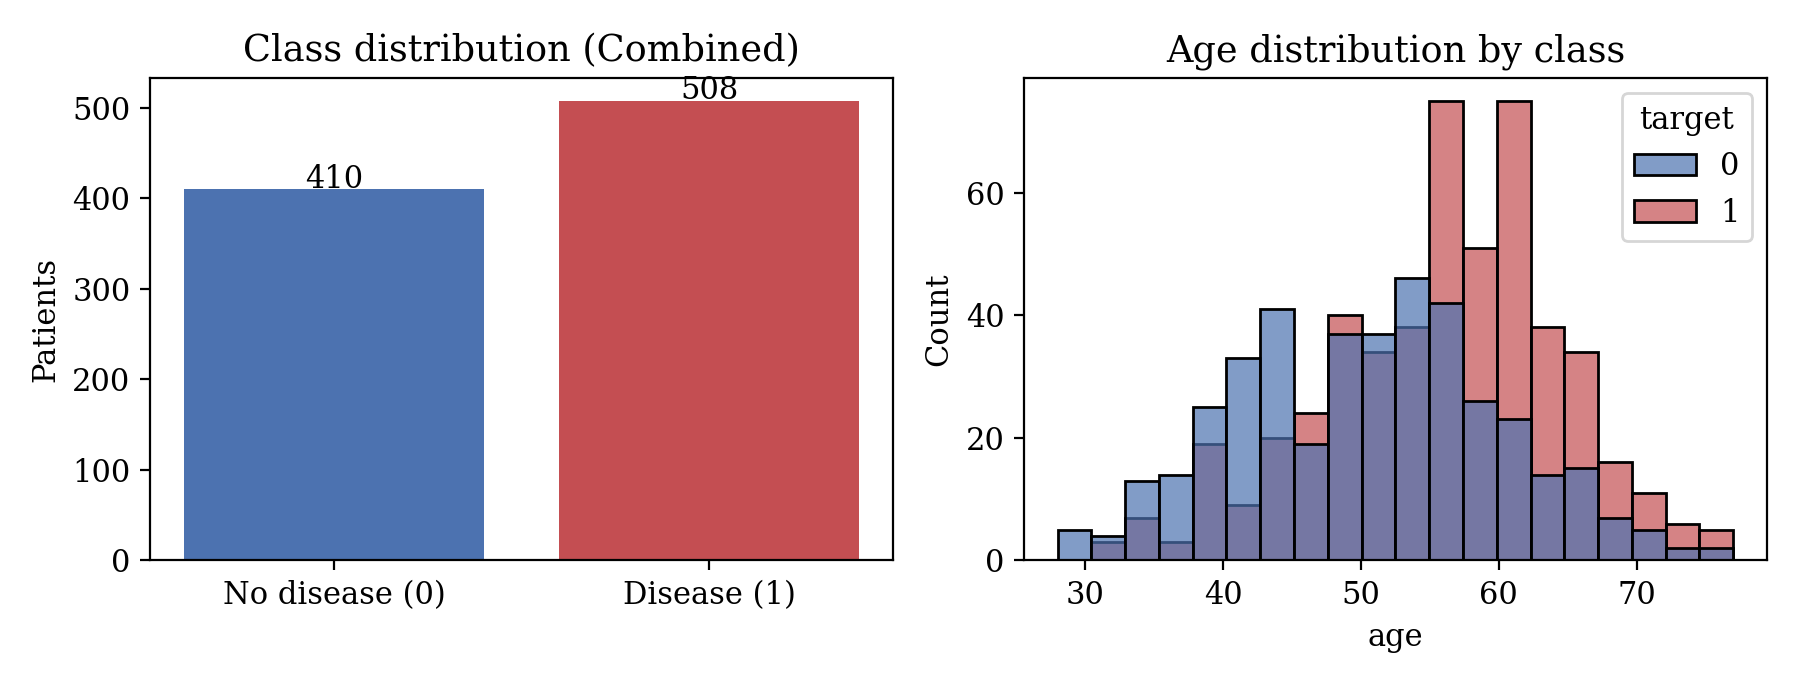
\includegraphics[width=0.62\textwidth]{figures/eda_combined.png}
\caption{Class balance and age distribution, Combined dataset}
\end{figure}

The correlation heat map of figure 3.4 shows that no pair of predictors is strongly correlated with each other (the largest absolute value is below 0.6), so the redundancy removal rule of the Pearson step never fires; the step acts purely as a relevance filter. The attributes most correlated with the label are thal, ca, exang, oldpeak, cp and thalach (negative) on Cleveland, and cp, exang, thalach and oldpeak on the combined data.

\begin{figure}[htbp]
\centering
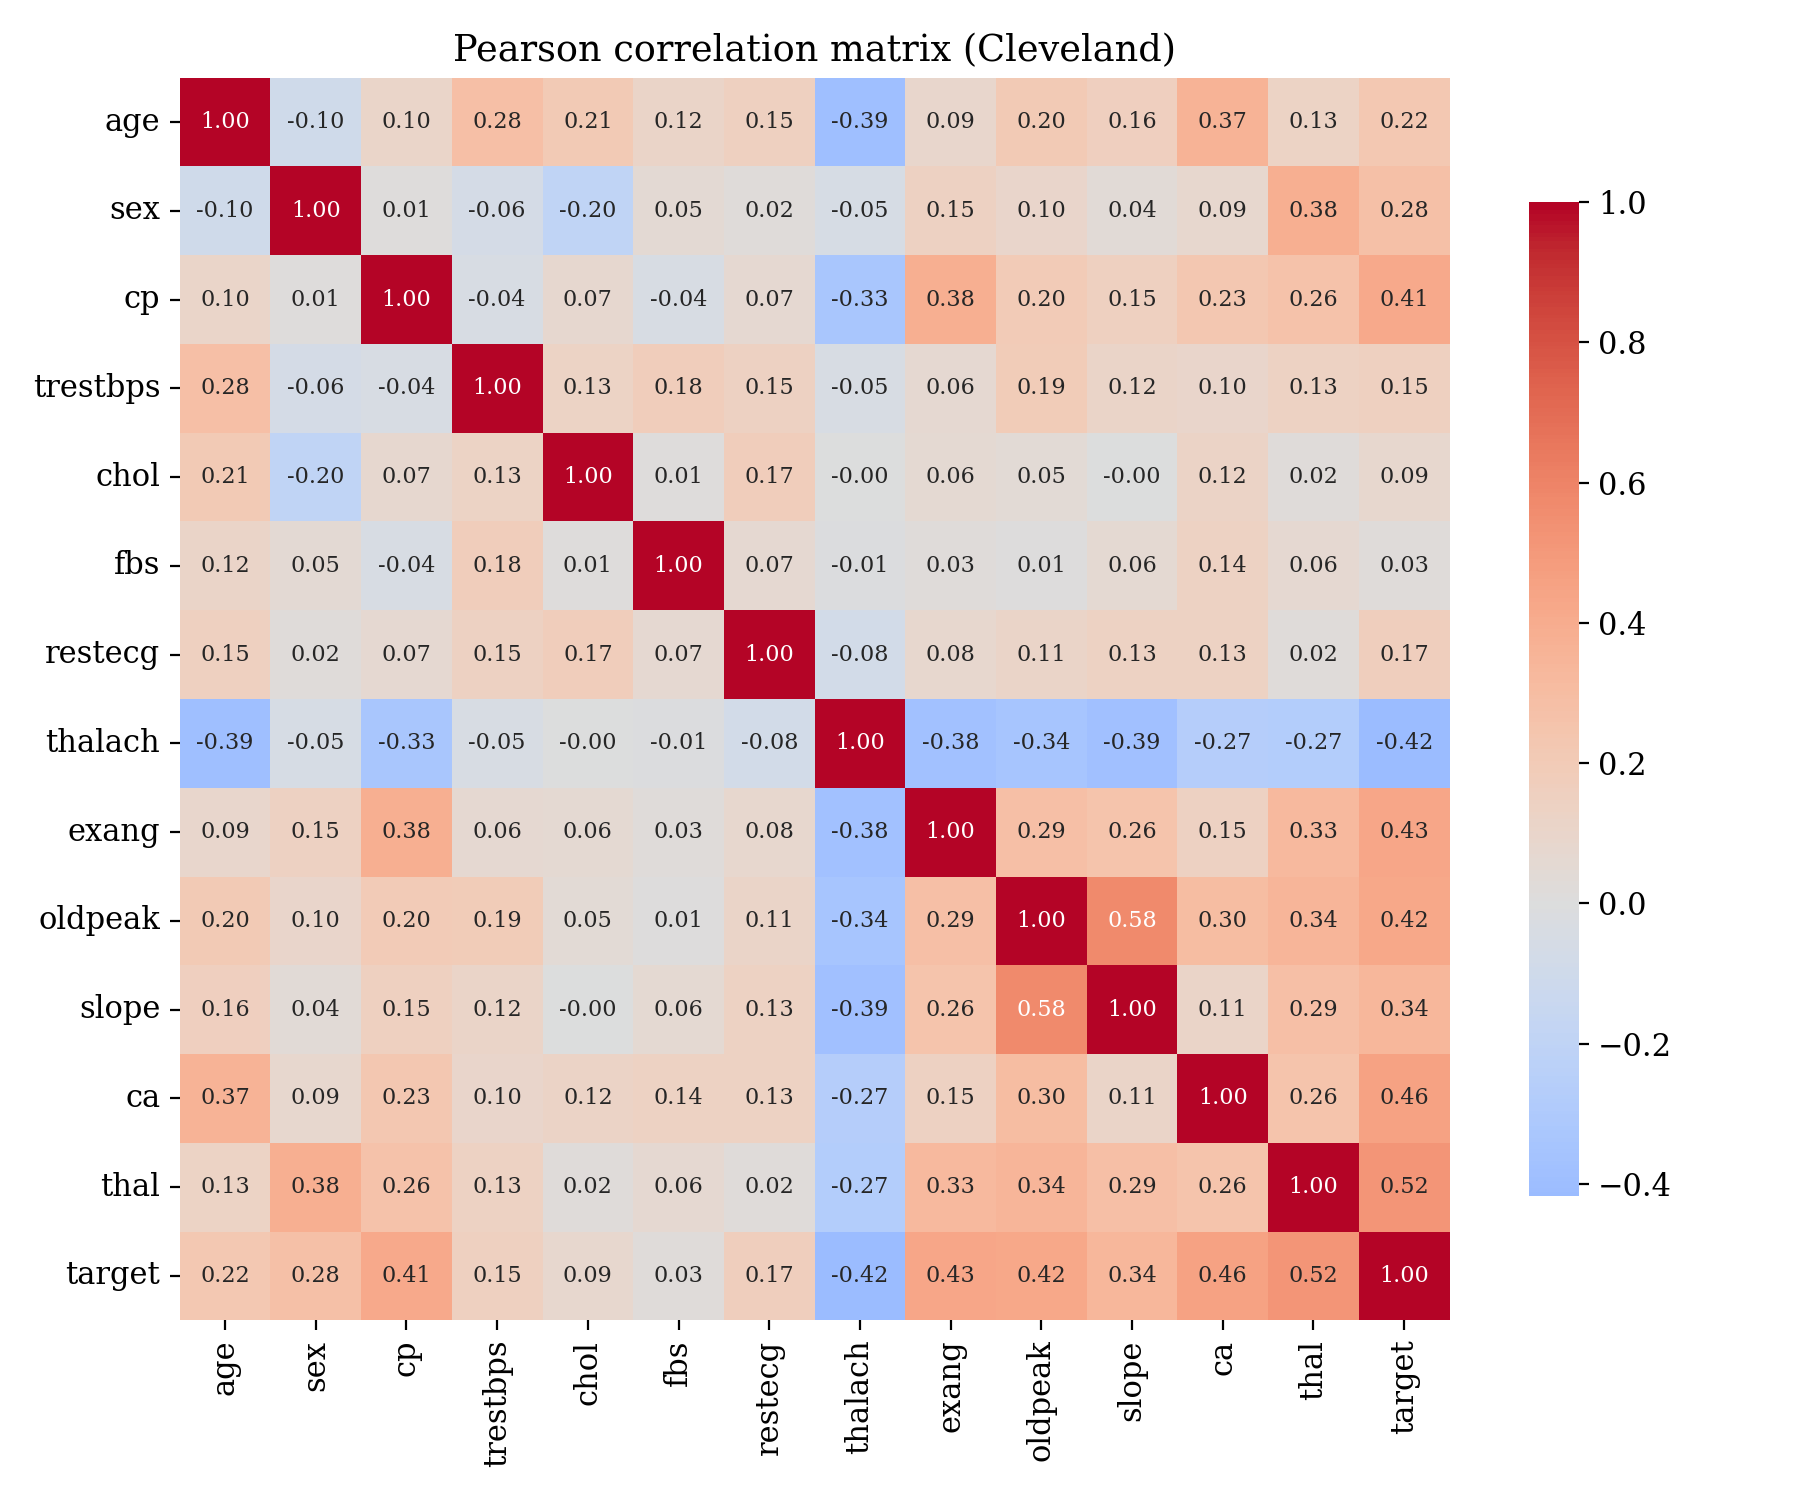
\includegraphics[width=0.56\textwidth]{figures/corr_cleveland.png}
\caption{Pearson correlation matrix, Cleveland (the combined dataset shows the same pattern)}
\end{figure}

\section{Feature Selection and Normalisation}
The base paper computes the \textbf{Pearson correlation coefficient} between attributes and removes highly correlated ones, but does not state the threshold. We make the rule explicit. For every predictor x and the label y,

\begin{equation}
r_{xy} = \frac{\operatorname{Cov}(x, y)}{\sigma_x \sigma_y} = \frac{\sum_i (x_i-\bar{x})(y_i-\bar{y})}{\sqrt{\sum_i (x_i-\bar{x})^2}\sqrt{\sum_i (y_i-\bar{y})^2}}
\end{equation}

where Cov(x, y) is the covariance (how much x and y move together), and the two standard deviations in the denominator rescale it to the range -1 to +1 so that r\_xy does not depend on the units of x. A predictor is \textbf{kept} if \textbar{}r\_xy\textbar{} is at least 0.10; if two kept predictors were correlated above 0.80 with each other, the one less correlated with the label would be dropped. On Cleveland this removes chol, fbs and keeps 11 attributes; on the combined data it removes chol, restecg. Figures 3.5 and 3.6 show the ranked correlations with the cut-off line.

\begin{figure}[htbp]
\centering
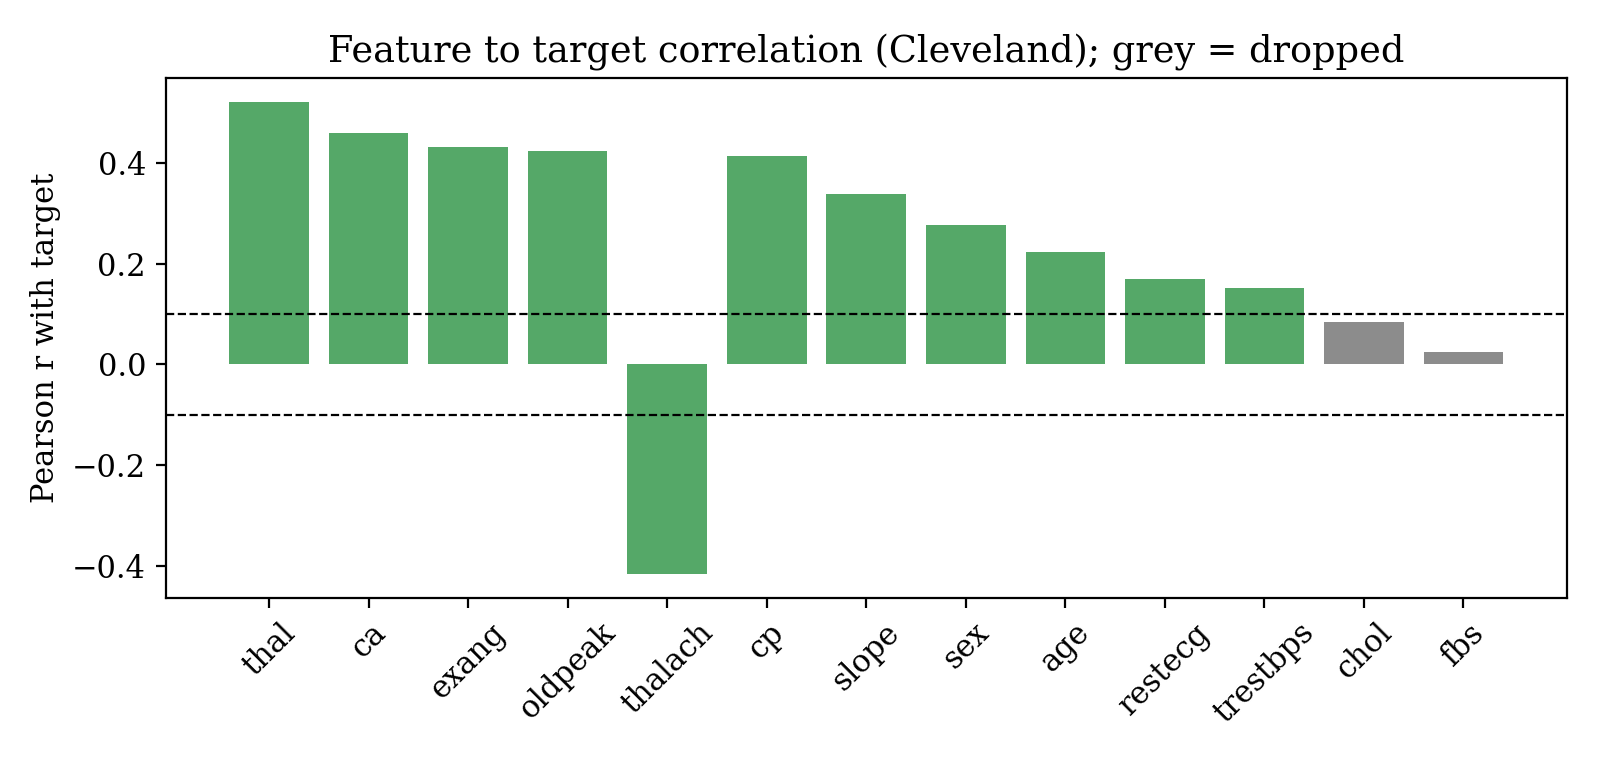
\includegraphics[width=0.60\textwidth]{figures/target_corr_cleveland.png}
\caption{Correlation of each attribute with the label, Cleveland (grey bars are dropped)}
\end{figure}

\begin{figure}[htbp]
\centering
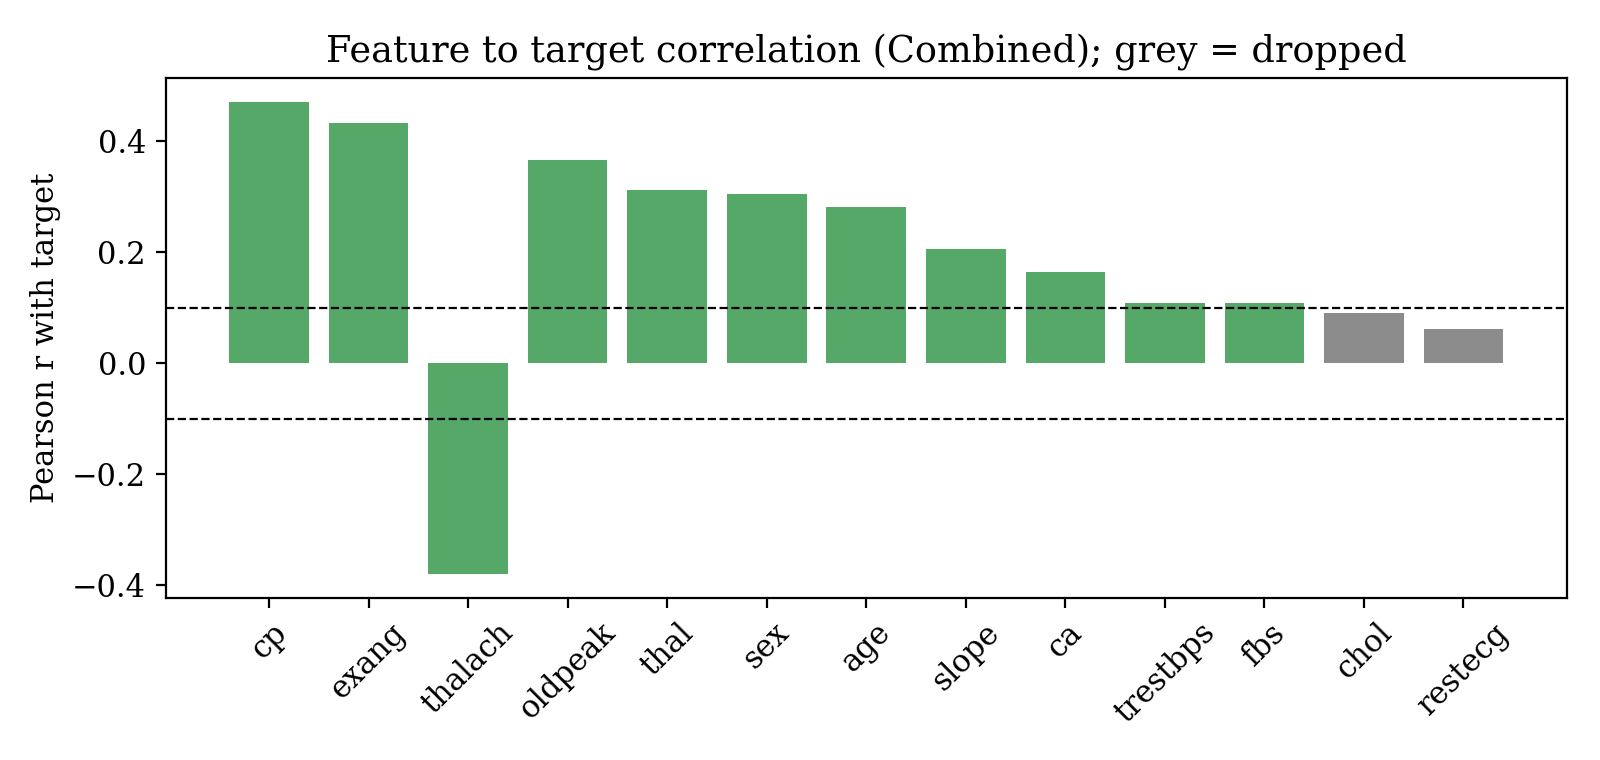
\includegraphics[width=0.60\textwidth]{figures/target_corr_combined.png}
\caption{Correlation of each attribute with the label, Combined dataset}
\end{figure}

\textbf{MinMax normalisation} maps every attribute to the interval 0 to 1:

\begin{equation}
x' = \frac{x - x_{\min}}{x_{\max} - x_{\min}}
\end{equation}

Here x\_min and x\_max are the minimum and maximum of that attribute \textbf{in the training fold}; subtracting x\_min shifts the smallest value to 0 and dividing by the range stretches the largest to 1. This matters for the SVM and KNN members, whose distance computations would otherwise be dominated by large valued attributes such as cholesterol; tree based members are unaffected by it.

\section{Algorithms}
\subsection{Base Learners}
\begin{itemize}
  \item \textbf{Decision Tree (CART):} recursively splits the data on the attribute and threshold that most reduce the Gini impurity G = 1 - sum(p\_k\textasciicircum{}2), where p\_k is the fraction of class k in a node. Unpruned trees fit the training data perfectly and therefore have high variance.
  \item \textbf{Random Forest:} a bagging ensemble of trees where each split considers only a random subset of attributes, which decorrelates the trees. Fifty trees are used inside MPBE and one hundred as a stand-alone baseline.
  \item \textbf{Gaussian Naive Bayes:} applies Bayes' theorem P(y\textbar{}x) proportional to P(y) times the product of P(x\_j\textbar{}y), assuming attributes are conditionally independent and normally distributed within each class.
  \item \textbf{Support Vector Machine (RBF kernel):} finds the maximum margin separating boundary in a kernel induced feature space; probability outputs are obtained by Platt scaling so that the SVM can take part in soft aggregation.
  \item \textbf{Logistic Regression and KNN (k = 7)} are added as extra single model baselines.
\end{itemize}

\subsection{The MPBE Ensemble (proposed model of [1], our implementation)}
For each of the four base learners C1 (DT), C2 (RF), C3 (NB) and C4 (SVM), a \textbf{BaggingClassifier} with n = 100 estimators is built. Each estimator is trained on a \textbf{bootstrap sample} of the training fold (the same size as the fold, drawn with replacement, so about 63\% of the distinct rows appear in any one sample). The bagged probability of disease from member k is the mean over its 100 estimators, and the final MPBE score is the mean over the four members:

\begin{equation}
P_{\text{MPBE}}(y=1\mid x) = \frac{1}{4}\sum_{k=1}^{4}\;\frac{1}{100}\sum_{b=1}^{100} P_{k,b}(y=1\mid x), \qquad \hat{y} = \mathbb{1}\left[P_{\text{MPBE}} \ge 0.5\right]
\end{equation}

The inner sum averages the 100 bootstrap models of one base learner (this is what reduces variance); the outer sum averages the four different learner families (this is what lets the strengths of one family cover the weaknesses of another). The indicator 1[.] turns the averaged probability into a class by thresholding at 0.5. The paper describes the aggregation as 'the mean score', which we read as this soft average rather than a hard majority vote; a hard voting ensemble is included separately for comparison.

\subsection{Comparison Ensembles}
\begin{itemize}
  \item \textbf{Bagging (DT, 100):} a homogeneous bagging ensemble of decision trees; isolates the effect of using four learner families instead of one.
  \item \textbf{Voting (soft / hard):} DT, RF, NB, SVM and LR trained once each on the full training fold (no bootstrapping) and combined by averaging probabilities (soft) or by majority (hard).
  \item \textbf{Stacking:} DT, RF, NB and SVM as level 0 learners; their out-of-fold predictions (5 inner folds) become the input of a Logistic Regression meta learner that learns how much to trust each member.
  \item \textbf{AdaBoost (100 rounds, learning rate 0.5):} sequentially reweights training rows so that each new stump concentrates on rows misclassified so far; the final vote weights each stump by log((1 - err)/err).
  \item \textbf{Gradient Boosting (100 trees, depth 3, learning rate 0.1):} each new tree fits the negative gradient of the log loss of the current ensemble, i.e. the residual errors.
  \item \textbf{XGBoost (100 trees, depth 3, learning rate 0.1, subsample 0.9) [25]:} a regularised, second order implementation of gradient boosting with column subsampling.
\end{itemize}

\chapter{Implementation (Steps / Procedure)}
\begin{enumerate}
  \item \textbf{Download} the five UCI files (processed.cleveland.data, processed.hungarian.data, processed.switzerland.data, processed.va.data, heart.dat) into data/.
  \item \textbf{Load} each file with the 14 canonical column names, convert '?' to NaN, binarise num into target, and for the combined dataset tag the source, remap Statlog labels, set zero cholesterol and blood pressure to NaN, concatenate and drop duplicate rows.
  \item \textbf{Impute} missing cells with the column median and save the prepared CSVs (cleveland\_prepared.csv, combined\_prepared.csv).
  \item \textbf{Explore}: plot class balance, age histograms and the full correlation matrix.
  \item \textbf{Select features} with the Pearson rule (\textbar{}r\textbar{} with label at least 0.10, inter-feature \textbar{}r\textbar{} below 0.80) and plot the ranked correlations.
  \item \textbf{Build the model zoo}: 14 models, each wrapped in Pipeline(MinMaxScaler, classifier) so scaling is fitted per fold.
  \item \textbf{Cross validate} every model with StratifiedKFold(10, shuffle=True, random\_state=42) and record accuracy, precision, recall, F1 and ROC-AUC per fold.
  \item \textbf{Hold-out evaluation}: one stratified 80:20 split (random\_state=42); fit every model, save confusion matrices, ROC curves and Random Forest feature importances.
  \item \textbf{Ablation}: repeat the MPBE cross validation on all 13 attributes to measure what the selection step contributes.
  \item \textbf{Repeat} steps 4 to 9 on the combined dataset and draw the cross dataset comparison chart.
  \item \textbf{GUI}: a Tkinter window loads the prepared data, trains MPBE once, and predicts for values typed by the user.
\end{enumerate}

The whole run (both datasets, all models, all figures) takes roughly eight minutes on a laptop CPU because MPBE trains 400 estimators per fold and the bagged SVM with probability calibration is the slowest member. The script caches results so that figures can be redrawn without retraining.

\chapter{Experimental Setup}
\section{Parameters}
\begin{table}[htbp]
\centering
\caption{Model parameters}
\footnotesize
\begin{tabular}{>{\raggedright\arraybackslash}p{0.251\textwidth}>{\raggedright\arraybackslash}p{0.689\textwidth}}
\hline
\textbf{Model} & \textbf{Setting} \\
\hline
MPBE & 4 x BaggingClassifier, n\_estimators = 100, bootstrap = True; bases DT(default), RF(50 trees), GaussianNB, SVC(rbf, probability=True); soft mean aggregation \\
Decision Tree & Gini criterion, no depth limit (scikit-learn defaults) \\
Random Forest & 100 trees, sqrt(features) per split \\
SVM & RBF kernel, C = 1, gamma = scale, Platt probabilities \\
Logistic Regression & L2 penalty, max\_iter = 1000 \\
KNN & k = 7, Euclidean distance \\
Voting & DT + RF + NB + SVM + LR, soft (probability mean) and hard (majority) \\
Stacking & DT, RF, NB, SVM level 0; Logistic Regression meta learner; 5 inner folds \\
AdaBoost & 100 decision stumps, learning rate 0.5 \\
Gradient Boosting & 100 trees, max\_depth 3, learning rate 0.1 \\
XGBoost & 100 trees, max\_depth 3, learning rate 0.1, subsample 0.9, colsample\_bytree 0.9, logloss \\
Feature selection & \textbar{}r(x, y)\textbar{} \textgreater{}= 0.10 keep; inter-feature \textbar{}r\textbar{} \textgreater{} 0.80 drop weaker \\
Validation & StratifiedKFold(10, shuffle) and stratified 80:20 hold-out; random\_state = 42 everywhere \\
\hline
\end{tabular}
\end{table}

\section{Tools}
Visual Studio Code / Jupyter for development, Git for versioning, a standard laptop CPU (no GPU is needed), and matplotlib for all figures. The desktop interface uses Tkinter, which ships with Python.

\section{Libraries}
\begin{table}[htbp]
\centering
\caption{Libraries and versions}
\footnotesize
\begin{tabular}{>{\raggedright\arraybackslash}p{0.272\textwidth}>{\raggedright\arraybackslash}p{0.146\textwidth}>{\raggedright\arraybackslash}p{0.522\textwidth}}
\hline
\textbf{Library} & \textbf{Version} & \textbf{Used for} \\
\hline
scikit-learn [24] & 1.8 & All classifiers except XGBoost, Pipeline, MinMaxScaler, StratifiedKFold, metrics \\
xgboost [25] & 3.4 & XGBClassifier \\
pandas & 3.0 & Data loading, cleaning, results tables \\
numpy & 2.x & Array operations, mean aggregation in MPBE \\
matplotlib / seaborn & 3.x / 0.13 & Figures \\
tkinter & built in & Desktop prediction window \\
\hline
\end{tabular}
\end{table}

\section{Framework}
scikit-learn's \textbf{estimator API} (fit, predict, predict\_proba) is the framework; MPBE is implemented as a class that follows it (ClassifierMixin, BaseEstimator) so it can be dropped into Pipeline and cross\_validate exactly like a built in model.

\section{Languages}
Python 3.12. LaTeX was used to typeset the paper and this report.

\chapter{Evaluation and Results / Discussion}
\section{Metrics}
With TP, TN, FP, FN the entries of the confusion matrix: \textbf{Accuracy} = (TP + TN) / (TP + TN + FP + FN) is the fraction of correct predictions; \textbf{Precision} = TP / (TP + FP) is the fraction of predicted patients who really have disease; \textbf{Recall} (sensitivity) = TP / (TP + FN) is the fraction of real patients the model catches, which is the clinically important number; \textbf{F1} = 2 x Precision x Recall / (Precision + Recall) is their harmonic mean, which is low if either is low; \textbf{ROC-AUC} is the probability that a randomly chosen diseased patient receives a higher score than a randomly chosen healthy one, computed as the area under the curve of true positive rate against false positive rate over all thresholds. Cross validation figures are means over the 10 folds with the standard deviation shown for accuracy.

\section{Results on the Cleveland Dataset}
\begin{table}[htbp]
\centering
\caption{10-fold stratified cross validation, Cleveland (303 records, 11 selected attributes)}
\footnotesize
\begin{tabular}{>{\raggedright\arraybackslash}p{0.300\textwidth}>{\raggedright\arraybackslash}p{0.176\textwidth}>{\raggedright\arraybackslash}p{0.134\textwidth}>{\raggedright\arraybackslash}p{0.124\textwidth}>{\raggedright\arraybackslash}p{0.114\textwidth}>{\raggedright\arraybackslash}p{0.093\textwidth}}
\hline
\textbf{Model} & \textbf{Accuracy (\%)} & \textbf{Precision (\%)} & \textbf{Recall (\%)} & \textbf{F1 (\%)} & \textbf{ROC-AUC} \\
\hline
Naive Bayes & 83.78 $\pm$ 6.10 & 85.19 & 79.07 & 81.66 & 0.902 \\
Stacking (LR meta) & 83.78 $\pm$ 6.79 & 85.37 & 79.07 & 81.55 & 0.915 \\
AdaBoost & 83.45 $\pm$ 5.44 & 84.35 & 79.84 & 81.65 & 0.910 \\
Voting (soft) & 82.84 $\pm$ 5.09 & 83.92 & 79.12 & 80.97 & 0.910 \\
Logistic Regression & 82.80 $\pm$ 7.01 & 83.66 & 78.35 & 80.69 & 0.908 \\
Voting (hard) & 82.48 $\pm$ 6.00 & 84.10 & 77.64 & 80.31 & n/a \\
MPBE (proposed, replicated) & 82.46 $\pm$ 6.41 & 84.30 & 76.92 & 80.03 & 0.912 \\
Random Forest & 82.17 $\pm$ 4.26 & 83.13 & 77.69 & 80.03 & 0.897 \\
SVM (RBF) & 82.15 $\pm$ 6.24 & 83.56 & 77.58 & 79.92 & 0.903 \\
XGBoost & 81.85 $\pm$ 4.72 & 83.57 & 76.98 & 79.69 & 0.899 \\
Gradient Boosting & 80.49 $\pm$ 5.67 & 80.30 & 76.87 & 78.30 & 0.874 \\
KNN (k=7) & 79.87 $\pm$ 5.02 & 78.37 & 79.07 & 78.17 & 0.877 \\
Bagging (DT, 100) & 79.83 $\pm$ 4.93 & 80.91 & 74.07 & 76.92 & 0.894 \\
Decision Tree & 77.17 $\pm$ 7.19 & 77.92 & 72.58 & 74.29 & 0.768 \\
\hline
\end{tabular}
\end{table}

\begin{figure}[htbp]
\centering
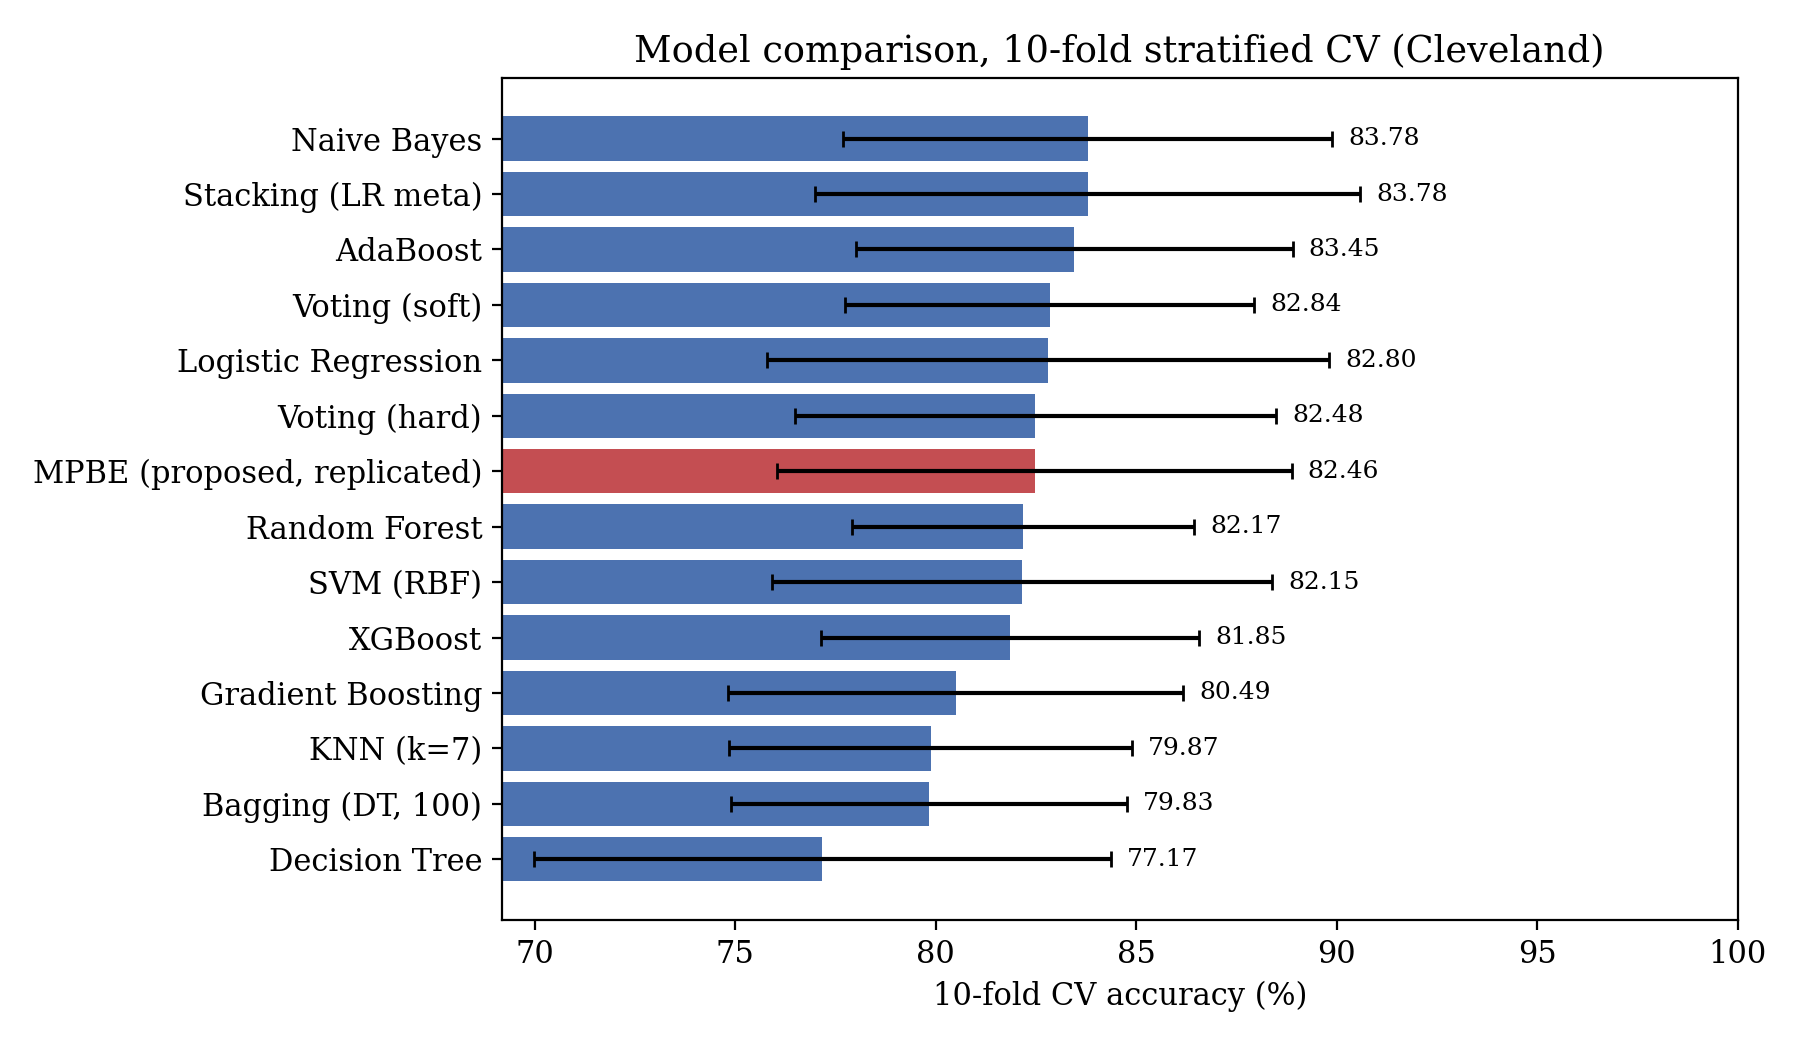
\includegraphics[width=0.62\textwidth]{figures/cv_accuracy_cleveland.png}
\caption{10-fold CV accuracy with standard deviation, Cleveland (MPBE in red)}
\end{figure}

MPBE reaches \textbf{82.46\% accuracy} and the \textbf{second highest ROC-AUC (0.912)} of all fourteen models, ranking 7th by accuracy. The differences between the top nine models (from 83.78\% down to about 82\%) are well inside one standard deviation (about 5 to 7 points on folds of 30 patients), so on this dataset they are statistically indistinguishable. What is clear is the gap to the single Decision Tree (77.2\%) and to homogeneous bagging of trees (79.8\%): mixing four learner families is worth about 2.5 points over bagging one family, which is exactly the argument of the base paper. Naive Bayes and Stacking tie for first by accuracy, and AdaBoost, soft Voting and Logistic Regression are essentially level with MPBE.

\begin{table}[htbp]
\centering
\caption{Stratified 80:20 hold-out, Cleveland (61 test patients)}
\footnotesize
\begin{tabular}{>{\raggedright\arraybackslash}p{0.300\textwidth}>{\raggedright\arraybackslash}p{0.176\textwidth}>{\raggedright\arraybackslash}p{0.134\textwidth}>{\raggedright\arraybackslash}p{0.124\textwidth}>{\raggedright\arraybackslash}p{0.114\textwidth}>{\raggedright\arraybackslash}p{0.093\textwidth}}
\hline
\textbf{Model} & \textbf{Accuracy (\%)} & \textbf{Precision (\%)} & \textbf{Recall (\%)} & \textbf{F1 (\%)} & \textbf{ROC-AUC} \\
\hline
Random Forest & 90.16 & 84.38 & 96.43 & 90.00 & 0.956 \\
AdaBoost & 88.52 & 86.21 & 89.29 & 87.72 & 0.972 \\
Voting (soft) & 86.89 & 79.41 & 96.43 & 87.10 & 0.942 \\
Stacking (LR meta) & 86.89 & 79.41 & 96.43 & 87.10 & 0.953 \\
MPBE (proposed, replicated) & 86.89 & 81.25 & 92.86 & 86.67 & 0.958 \\
Naive Bayes & 86.89 & 79.41 & 96.43 & 87.10 & 0.952 \\
Voting (hard) & 85.25 & 78.79 & 92.86 & 85.25 & 0.858 \\
Bagging (DT, 100) & 85.25 & 77.14 & 96.43 & 85.71 & 0.949 \\
XGBoost & 85.25 & 77.14 & 96.43 & 85.71 & 0.963 \\
Gradient Boosting & 83.61 & 76.47 & 92.86 & 83.87 & 0.952 \\
Logistic Regression & 81.97 & 77.42 & 85.71 & 81.36 & 0.942 \\
SVM (RBF) & 80.33 & 76.67 & 82.14 & 79.31 & 0.930 \\
Decision Tree & 77.05 & 70.59 & 85.71 & 77.42 & 0.777 \\
KNN (k=7) & 75.41 & 69.70 & 82.14 & 75.41 & 0.870 \\
\hline
\end{tabular}
\end{table}

\begin{figure}[htbp]
\centering
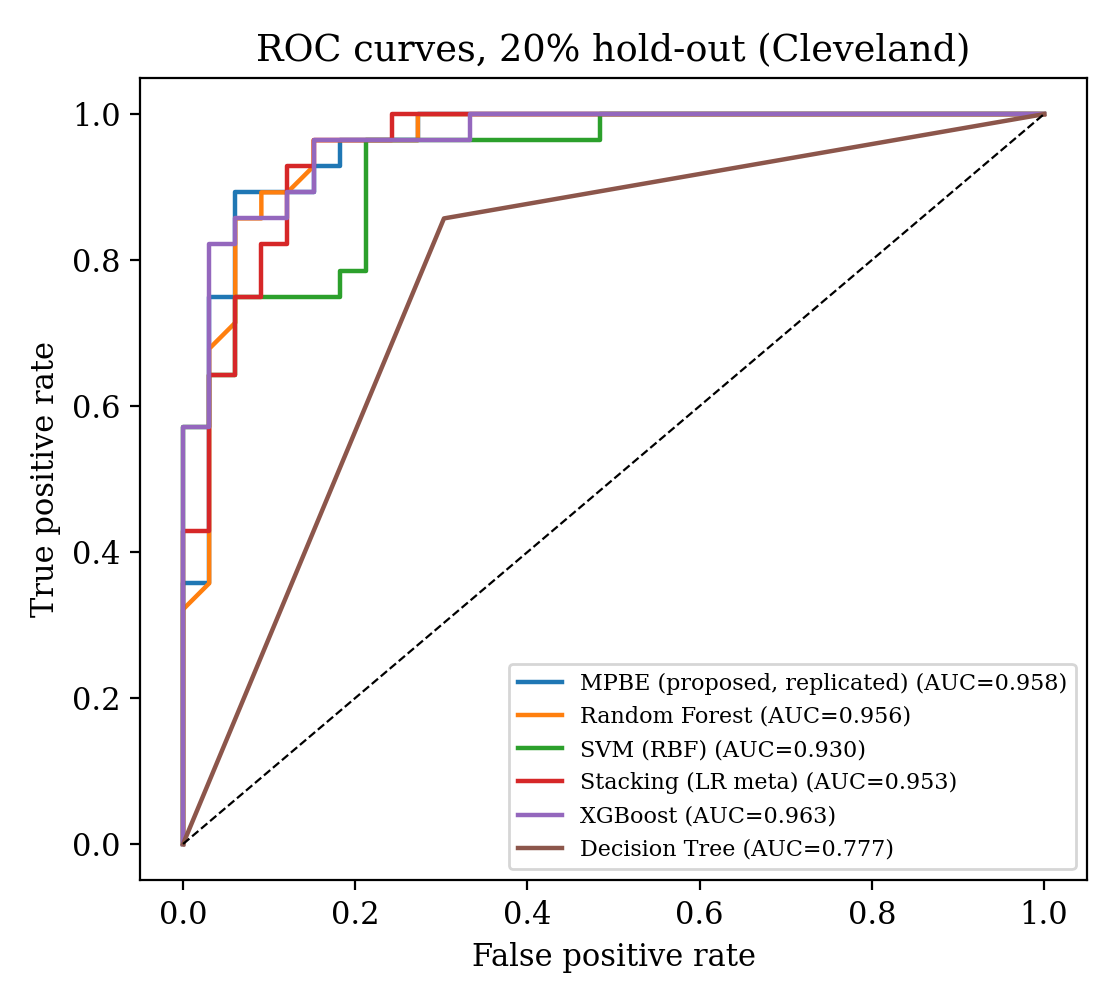
\includegraphics[width=0.40\textwidth]{figures/roc_cleveland.png}
\caption{ROC curves on the hold-out split, Cleveland}
\end{figure}

\begin{figure}[htbp]
\centering
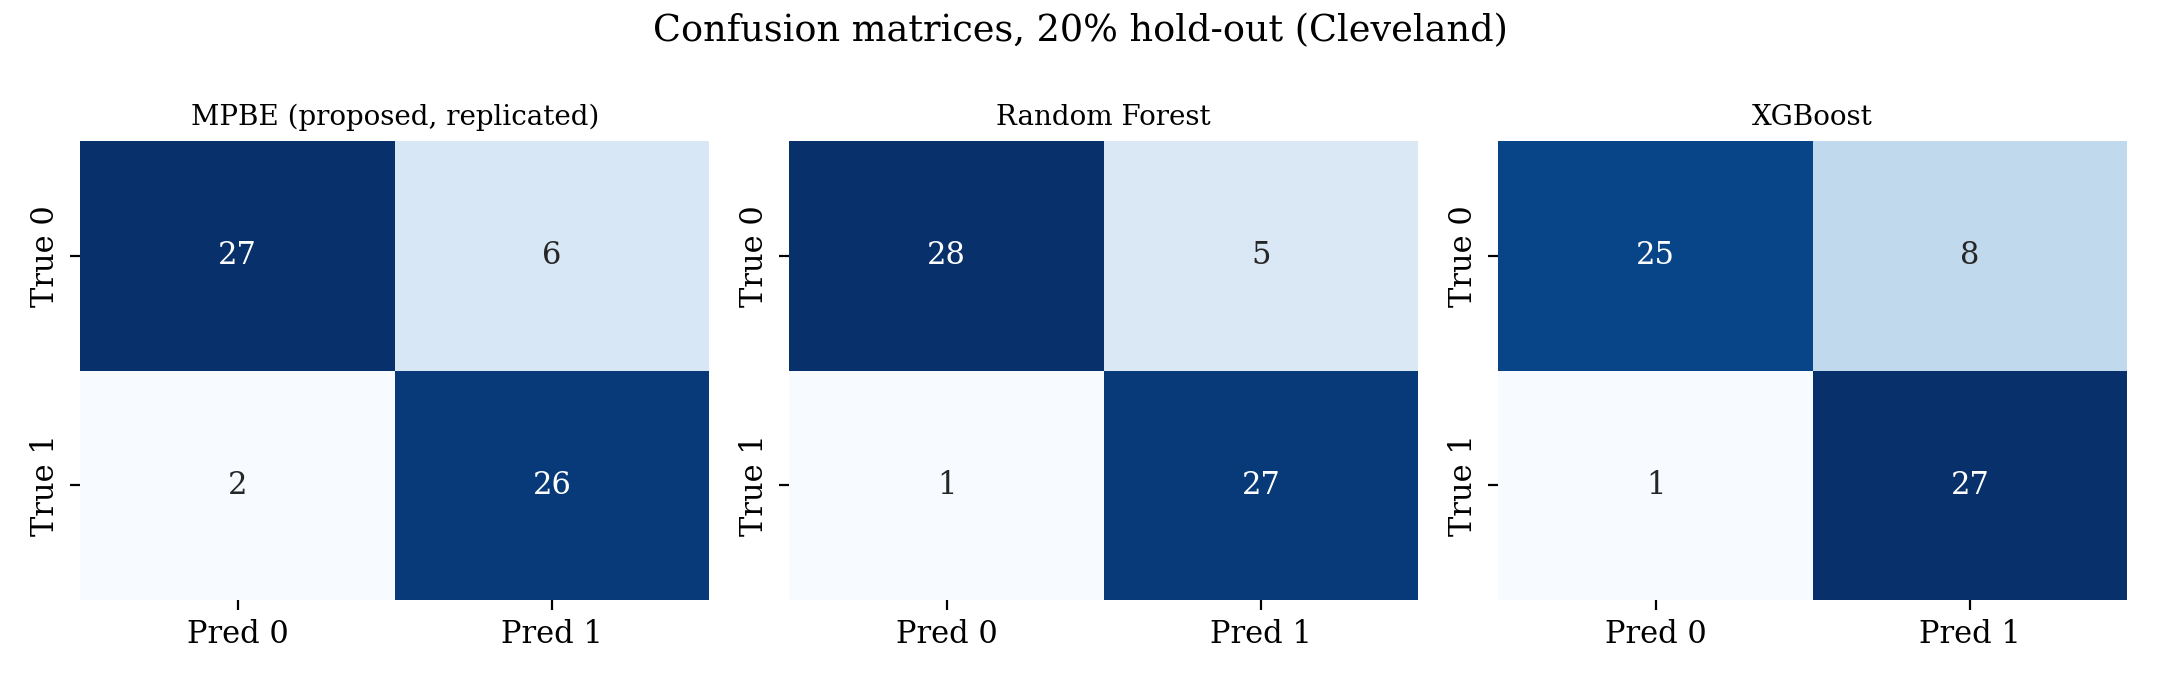
\includegraphics[width=0.70\textwidth]{figures/cm_cleveland.png}
\caption{Confusion matrices on the hold-out split, Cleveland}
\end{figure}

On the single hold-out split MPBE scores 86.89\% with recall 92.86\% and AUC 0.958: it misses only 2 of the 28 diseased patients. The 61 patient test set is small enough that a single patient is 1.6 points of accuracy, which is why the hold-out ranking (Random Forest first at 90.2\%) differs from the cross validated one. This is also the most likely explanation of the 95.33\% in [1]: a favourable single split, plus scaling and feature selection performed on the whole dataset before splitting. Under a leakage free 10-fold protocol no model in our study exceeds 84\% mean accuracy, which is consistent with [8], [9], [10] and [21].

\section{Results on the Combined Dataset}
\begin{table}[htbp]
\centering
\caption{10-fold stratified cross validation, Combined dataset (918 records, 11 selected attributes)}
\footnotesize
\begin{tabular}{>{\raggedright\arraybackslash}p{0.300\textwidth}>{\raggedright\arraybackslash}p{0.176\textwidth}>{\raggedright\arraybackslash}p{0.134\textwidth}>{\raggedright\arraybackslash}p{0.124\textwidth}>{\raggedright\arraybackslash}p{0.114\textwidth}>{\raggedright\arraybackslash}p{0.093\textwidth}}
\hline
\textbf{Model} & \textbf{Accuracy (\%)} & \textbf{Precision (\%)} & \textbf{Recall (\%)} & \textbf{F1 (\%)} & \textbf{ROC-AUC} \\
\hline
MPBE (proposed, replicated) & 80.84 $\pm$ 3.53 & 82.42 & 83.29 & 82.81 & 0.884 \\
Random Forest & 80.73 $\pm$ 2.93 & 81.58 & 84.47 & 82.90 & 0.870 \\
Gradient Boosting & 80.72 $\pm$ 2.90 & 81.39 & 84.65 & 82.89 & 0.878 \\
Voting (hard) & 80.51 $\pm$ 3.23 & 82.91 & 82.10 & 82.38 & n/a \\
Stacking (LR meta) & 80.40 $\pm$ 3.49 & 81.67 & 83.69 & 82.56 & 0.883 \\
Logistic Regression & 80.19 $\pm$ 3.35 & 81.95 & 82.70 & 82.24 & 0.876 \\
Voting (soft) & 80.19 $\pm$ 3.65 & 82.22 & 82.30 & 82.18 & 0.877 \\
Naive Bayes & 80.18 $\pm$ 2.90 & 84.32 & 79.15 & 81.52 & 0.874 \\
AdaBoost & 80.18 $\pm$ 3.67 & 81.98 & 82.89 & 82.23 & 0.878 \\
SVM (RBF) & 79.75 $\pm$ 3.37 & 80.19 & 84.86 & 82.31 & 0.879 \\
XGBoost & 79.52 $\pm$ 2.54 & 80.71 & 83.08 & 81.75 & 0.878 \\
Bagging (DT, 100) & 79.52 $\pm$ 3.25 & 81.35 & 82.09 & 81.62 & 0.851 \\
KNN (k=7) & 78.22 $\pm$ 3.25 & 80.34 & 81.30 & 80.57 & 0.852 \\
Decision Tree & 70.81 $\pm$ 4.16 & 74.82 & 71.24 & 72.86 & 0.712 \\
\hline
\end{tabular}
\end{table}

\begin{figure}[htbp]
\centering
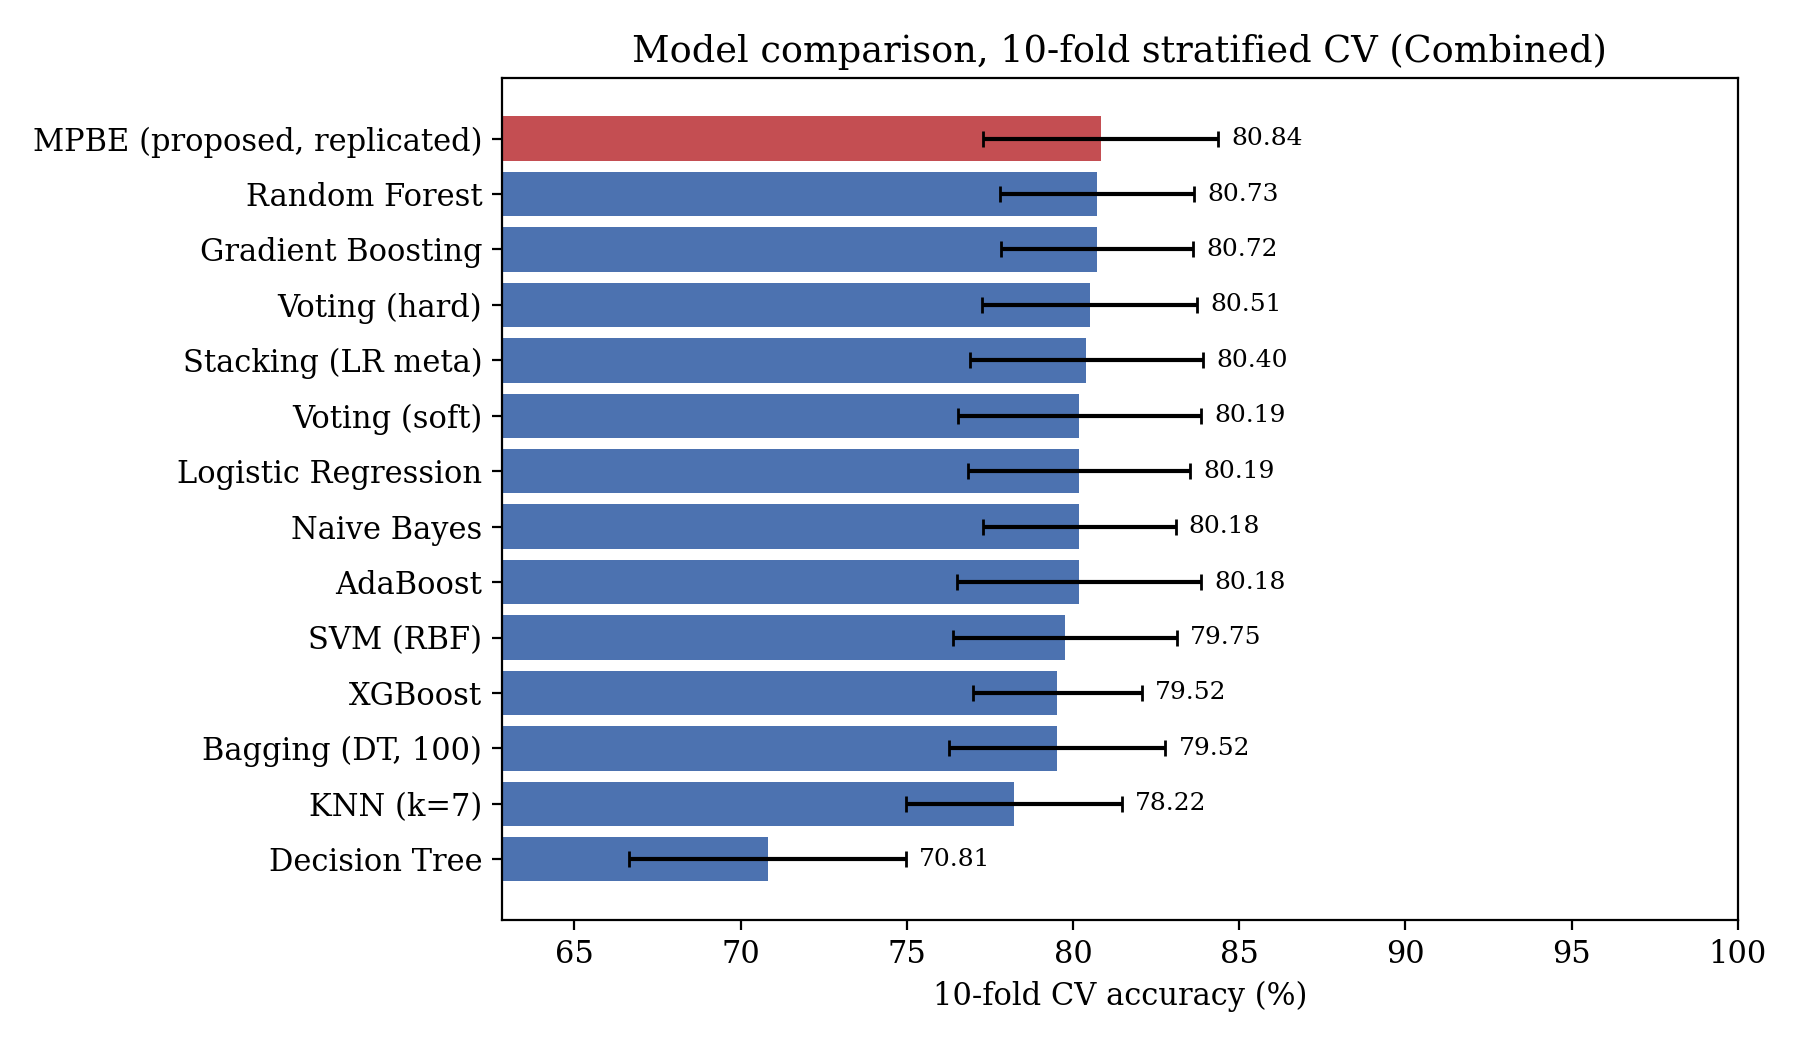
\includegraphics[width=0.62\textwidth]{figures/cv_accuracy_combined.png}
\caption{10-fold CV accuracy with standard deviation, Combined dataset}
\end{figure}

On the larger and noisier combined population \textbf{MPBE is the best model} by accuracy (80.84\%) and ties for the best ROC-AUC (0.884) with Stacking. The standard deviations shrink to about 3 points because each fold now holds 92 patients, so the ranking is more trustworthy than on Cleveland. Absolute accuracy is lower for every model because a third of the records come from hospitals whose protocols left slope, ca and thal mostly unrecorded (they were median imputed). The single Decision Tree drops to 70.8\%, so the value of ensembling grows as the data gets harder: MPBE is 10 points above its weakest member here versus 5 points on Cleveland.

\begin{table}[htbp]
\centering
\caption{Stratified 80:20 hold-out, Combined dataset (184 test patients)}
\footnotesize
\begin{tabular}{>{\raggedright\arraybackslash}p{0.300\textwidth}>{\raggedright\arraybackslash}p{0.176\textwidth}>{\raggedright\arraybackslash}p{0.134\textwidth}>{\raggedright\arraybackslash}p{0.124\textwidth}>{\raggedright\arraybackslash}p{0.114\textwidth}>{\raggedright\arraybackslash}p{0.093\textwidth}}
\hline
\textbf{Model} & \textbf{Accuracy (\%)} & \textbf{Precision (\%)} & \textbf{Recall (\%)} & \textbf{F1 (\%)} & \textbf{ROC-AUC} \\
\hline
MPBE (proposed, replicated) & 82.07 & 82.86 & 85.29 & 84.06 & 0.892 \\
Stacking (LR meta) & 81.52 & 82.08 & 85.29 & 83.65 & 0.891 \\
Voting (soft) & 80.98 & 81.31 & 85.29 & 83.25 & 0.880 \\
AdaBoost & 80.98 & 81.90 & 84.31 & 83.09 & 0.902 \\
SVM (RBF) & 80.98 & 79.65 & 88.24 & 83.72 & 0.880 \\
Gradient Boosting & 80.98 & 80.73 & 86.27 & 83.41 & 0.893 \\
XGBoost & 80.98 & 80.18 & 87.25 & 83.57 & 0.893 \\
Logistic Regression & 80.43 & 81.73 & 83.33 & 82.52 & 0.883 \\
Voting (hard) & 80.43 & 81.13 & 84.31 & 82.69 & 0.800 \\
Random Forest & 79.89 & 80.95 & 83.33 & 82.13 & 0.878 \\
Bagging (DT, 100) & 79.89 & 79.28 & 86.27 & 82.63 & 0.864 \\
Naive Bayes & 79.35 & 82.65 & 79.41 & 81.00 & 0.870 \\
KNN (k=7) & 78.80 & 80.00 & 82.35 & 81.16 & 0.877 \\
Decision Tree & 70.65 & 71.43 & 78.43 & 74.77 & 0.700 \\
\hline
\end{tabular}
\end{table}

\begin{figure}[htbp]
\centering
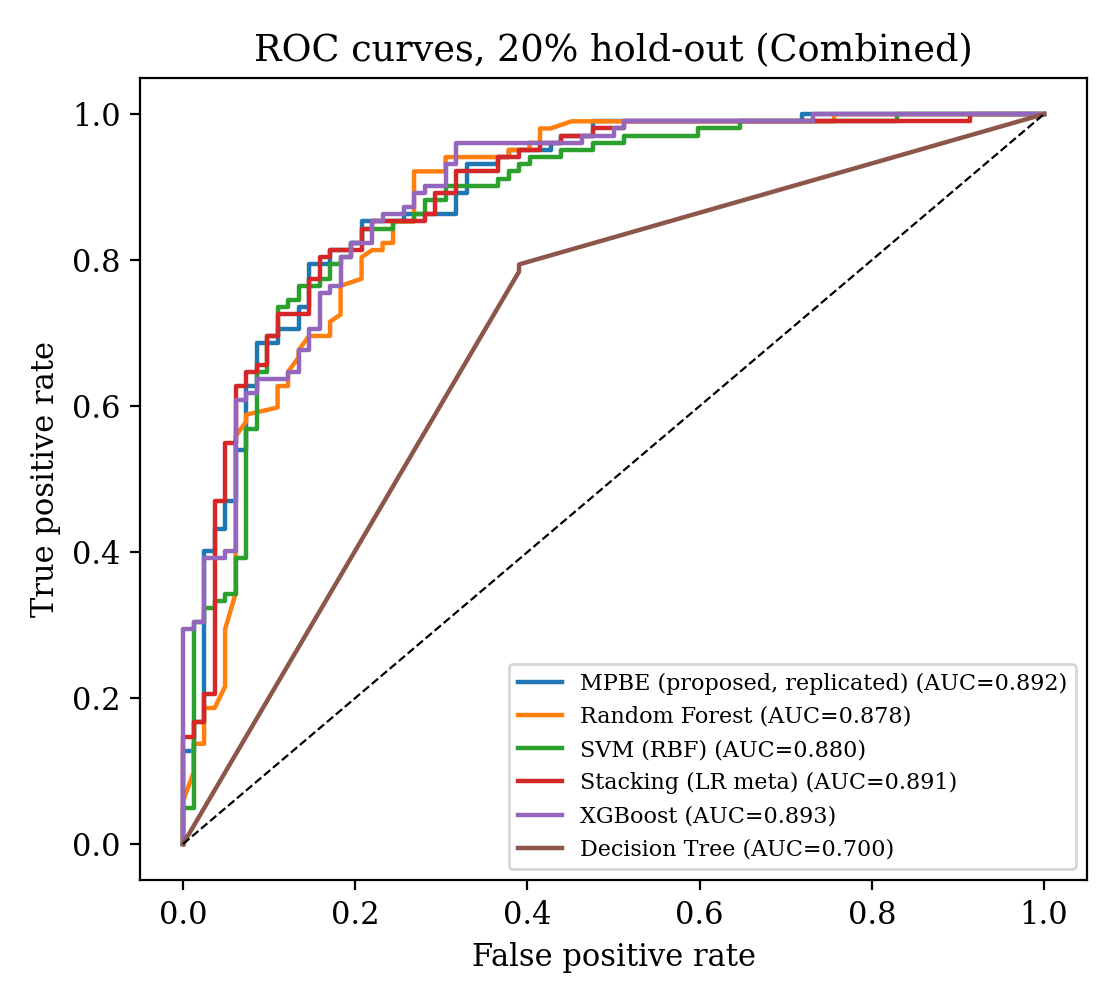
\includegraphics[width=0.40\textwidth]{figures/roc_combined.png}
\caption{ROC curves on the hold-out split, Combined dataset}
\end{figure}

\begin{figure}[htbp]
\centering
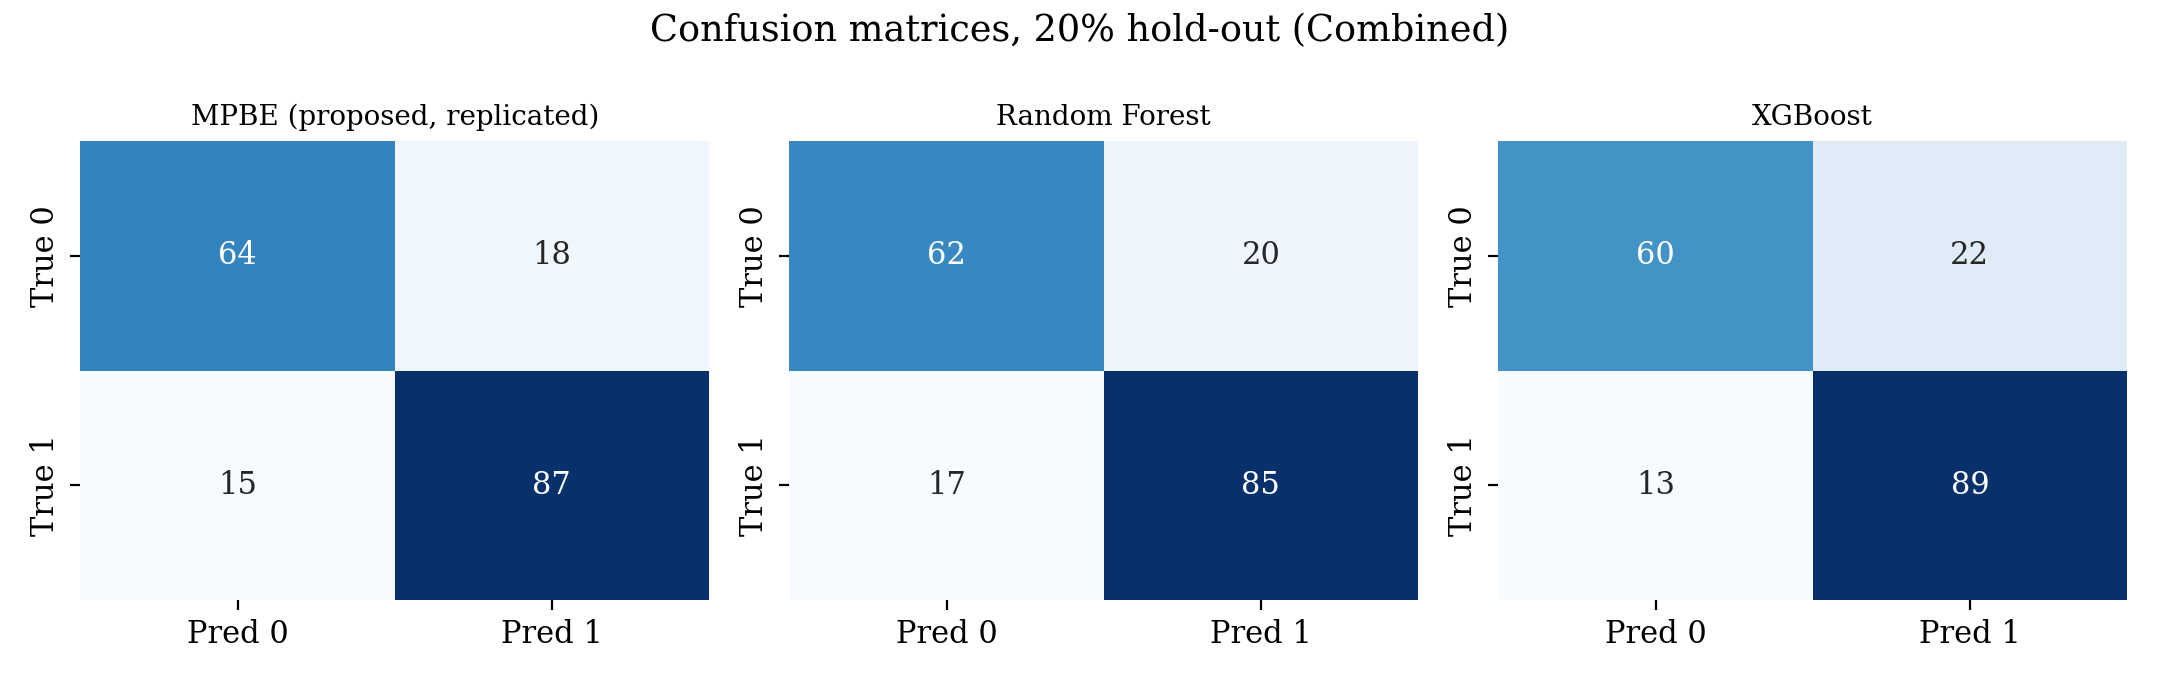
\includegraphics[width=0.70\textwidth]{figures/cm_combined.png}
\caption{Confusion matrices on the hold-out split, Combined dataset}
\end{figure}

MPBE is also first on the hold-out split (82.07\%, recall 85.29\%). AdaBoost has the highest AUC (0.90) but slightly lower accuracy at the 0.5 threshold, which suggests that threshold tuning could give it back a point or two; we kept the default threshold for all models to keep the comparison fair.

\section{Effect of Feature Selection (Ablation)}
\begin{table}[htbp]
\centering
\caption{MPBE with and without Pearson feature selection (10-fold CV)}
\footnotesize
\begin{tabular}{>{\raggedright\arraybackslash}p{0.188\textwidth}>{\raggedright\arraybackslash}p{0.188\textwidth}>{\raggedright\arraybackslash}p{0.188\textwidth}>{\raggedright\arraybackslash}p{0.188\textwidth}>{\raggedright\arraybackslash}p{0.188\textwidth}}
\hline
\textbf{Dataset} & \textbf{Attributes} & \textbf{Accuracy (\%)} & \textbf{F1 (\%)} & \textbf{ROC-AUC} \\
\hline
Cleveland & 11 selected & 82.46 & 80.03 & 0.912 \\
Cleveland & all 13 & 82.46 & 80.14 & 0.909 \\
Combined & 11 selected & 80.84 & 82.81 & 0.884 \\
Combined & all 13 & 81.05 & 82.89 & 0.888 \\
\hline
\end{tabular}
\end{table}

Removing the two weakest attributes changes accuracy by less than half a point in either direction and raises AUC by 0.003 on Cleveland. The \textbf{Pearson step is therefore harmless but not decisive}; its practical benefit is a slightly cheaper model (two fewer inputs, which for a screening tool means two fewer measurements) rather than higher accuracy. This agrees with [9] and [7], where feature selection added at most one or two points.

\section{Feature Importance}
\begin{figure}[htbp]
\centering
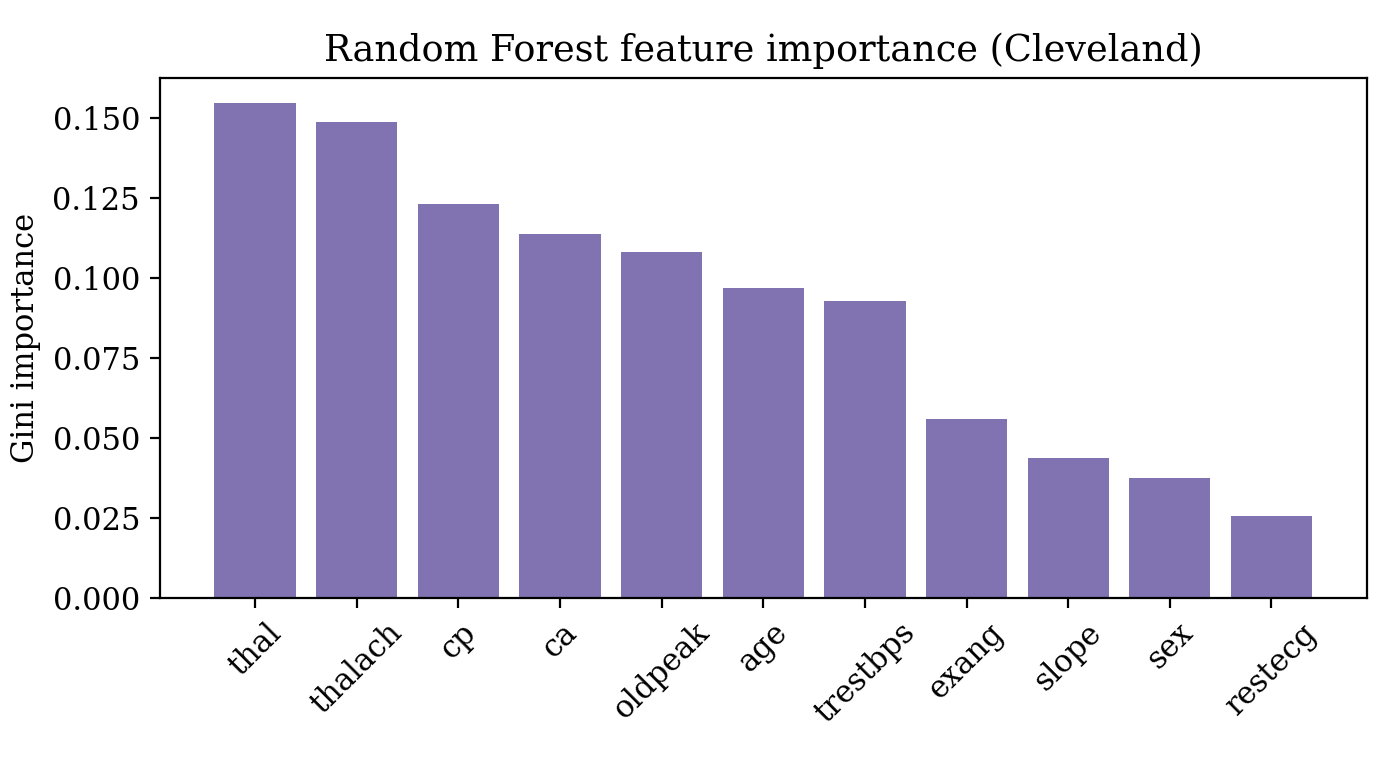
\includegraphics[width=0.55\textwidth]{figures/importance_cleveland.png}
\caption{Random Forest Gini importance of the selected attributes, Cleveland}
\end{figure}

\begin{figure}[htbp]
\centering
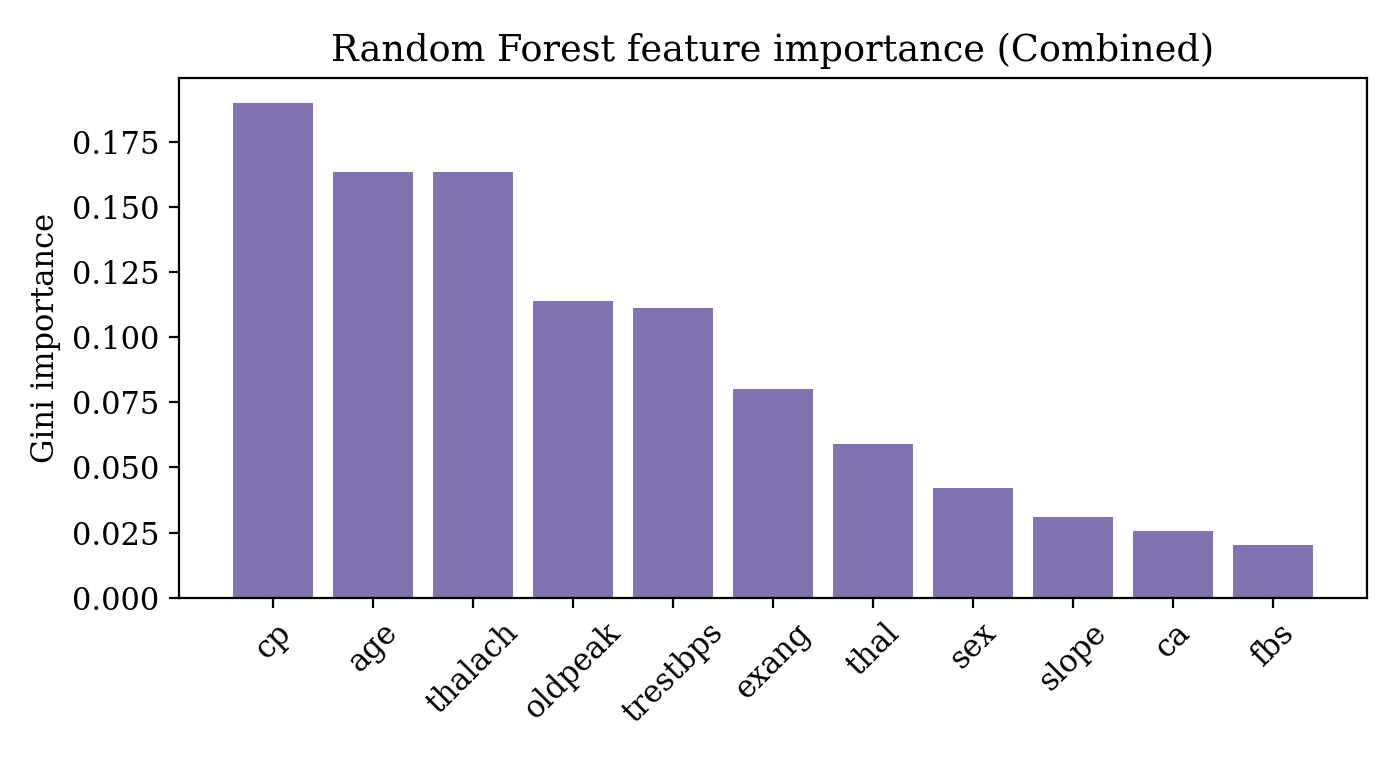
\includegraphics[width=0.55\textwidth]{figures/importance_combined.png}
\caption{Random Forest Gini importance of the selected attributes, Combined dataset}
\end{figure}

On Cleveland the Random Forest relies most on thal, thalach, cp, ca and oldpeak; on the combined data cp, age, thalach and oldpeak dominate while thal and ca lose importance because they are largely imputed outside Cleveland. Chest pain type, maximum heart rate and exercise ST depression are therefore the attributes a clinician would want recorded first, which agrees with [15] and [16].

\section{Cross Dataset Comparison}
\begin{figure}[htbp]
\centering
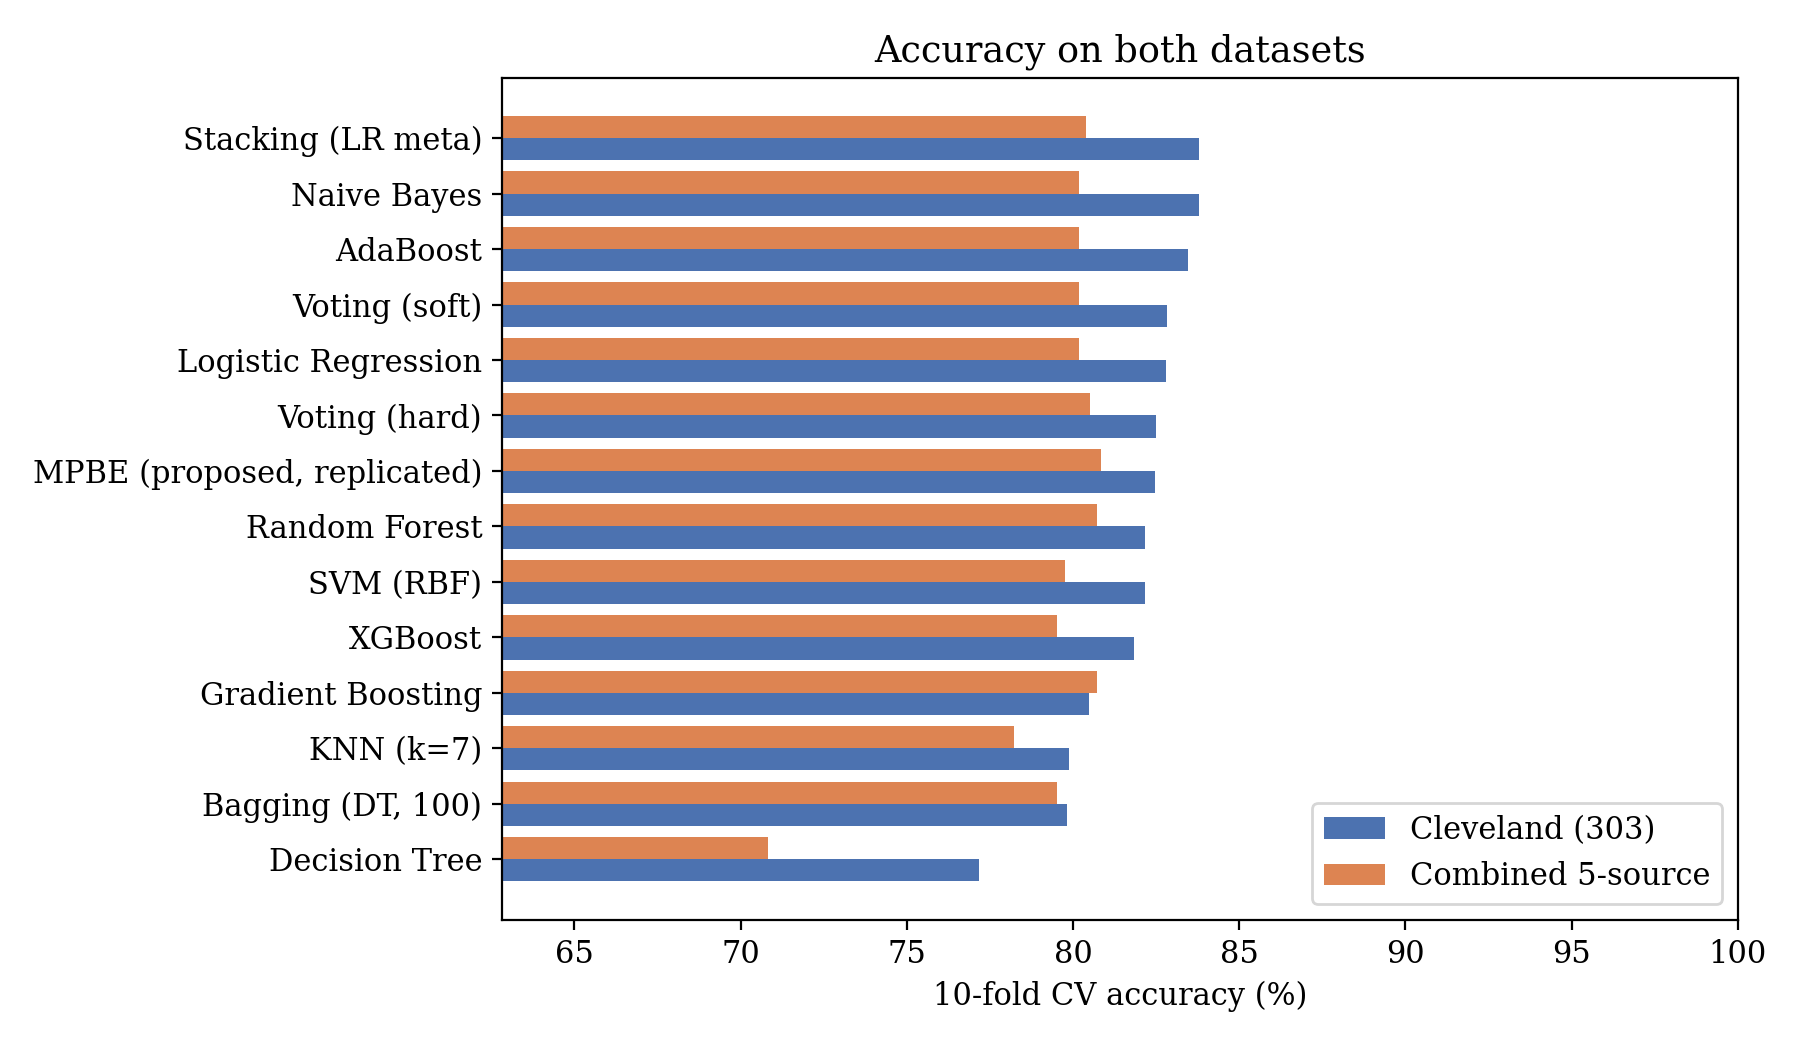
\includegraphics[width=0.62\textwidth]{figures/cross_dataset.png}
\caption{10-fold CV accuracy of every model on both datasets}
\end{figure}

Every model loses 1 to 7 points when moving from Cleveland to the combined population, and the loss is largest for the models that leaned on thal and ca. MPBE loses only about 1.6 points and moves from mid table to first place, which is the behaviour one wants from a model meant for deployment across hospitals: \textbf{stable rather than spectacular}.

\chapter{Graphical User Interface}
A minimal desktop interface was written with \textbf{Tkinter} (src/gui\_tkinter.py). On start it loads cleveland\_prepared.csv, applies the same Pearson selection, fits Pipeline(MinMaxScaler, MPBE) once (about 20 seconds), and then shows one entry field per selected attribute with the Cleveland median as default. Pressing Predict displays the ensemble probability of disease and the class, coloured green or red. No web server or browser is required; the window is shown in figure 7.1.

\begin{figure}[htbp]
\centering
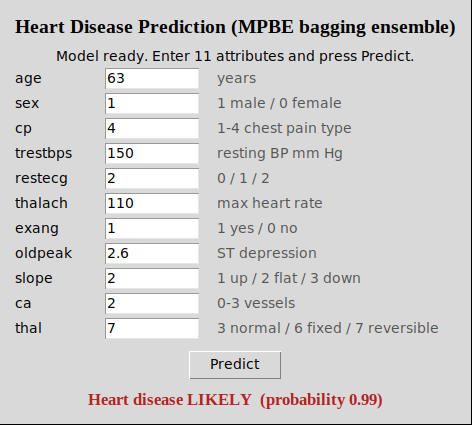
\includegraphics[width=0.38\textwidth]{figures/gui_screenshot.png}
\caption{Tkinter prediction window with an example patient}
\end{figure}

\chapter{Code}
\section{Libraries and Functions Used}
\begin{table}[htbp]
\centering
\caption{Main functions in heart\_ensemble.py}
\footnotesize
\begin{tabular}{>{\raggedright\arraybackslash}p{0.334\textwidth}>{\raggedright\arraybackslash}p{0.606\textwidth}}
\hline
\textbf{Function / class} & \textbf{Purpose} \\
\hline
load\_cleveland(), load\_combined() & Read the UCI files, binarise the label, clean impossible zeros, remove duplicates \\
preprocess(df) & Median imputation; returns the missing value count per column \\
pearson\_select(df, 0.10, 0.80) & Pearson relevance filter and redundancy rule; returns kept and dropped attributes \\
class MPBE & The proposed ensemble: four bagging members, soft mean aggregation; scikit-learn compatible \\
build\_models() & The 14 model zoo, each wrapped in Pipeline(MinMaxScaler, clf) \\
evaluate\_cv(), evaluate\_holdout() & Stratified 10-fold CV and 80:20 hold-out with all metrics, ROC data, confusion matrices and importances \\
fig\_*() & All figures used in this report \\
run\_dataset(df, tag, title) & Runs the whole procedure of chapter 4 for one dataset and writes results/summary\_\textless{}tag\textgreater{}.json \\
\hline
\end{tabular}
\end{table}

\section{Core Code Listing}
The complete script is about 500 lines. The two listings below define the method itself: the Pearson selection rule and the MPBE ensemble class. The full file, the Colab notebook and the GUI are submitted alongside this report.

\begin{lstlisting}[caption={Pearson correlation feature selection},]
def pearson_select(df, min_target_corr=0.10, max_inter_corr=0.80):
    """
    Keep a feature if |corr(feature, target)| >= min_target_corr.
    Additionally, if two kept features are correlated above max_inter_corr,
    drop the one less correlated with the target (redundancy removal,
    which is what the original paper means by 'highly correlated features
    are removed').
    """
    corr_t = df[FEATURES + ["target"]].corr()["target"].drop("target")
    keep = [f for f in FEATURES if abs(corr_t[f]) >= min_target_corr]
    inter = df[keep].corr().abs()
    dropped_redundant = []
    for i, a in enumerate(keep):
        for b in keep[i + 1:]:
            if a in dropped_redundant or b in dropped_redundant:
                continue
            if inter.loc[a, b] > max_inter_corr:
                weaker = a if abs(corr_t[a]) < abs(corr_t[b]) else b
                dropped_redundant.append(weaker)
    keep = [f for f in keep if f not in dropped_redundant]
    dropped = [f for f in FEATURES if f not in keep]
    return keep, dropped, corr_t
\end{lstlisting}

\begin{lstlisting}[caption={The MPBE ensemble class},]
class MPBE(ClassifierMixin, BaseEstimator):
    """
    MinMax normalized - Pearson coefficient Bagging Ensemble.
    Four bagging ensembles (100 bootstrap estimators each) are built, one per
    base learner (Decision Tree, Random Forest, Naive Bayes, SVM). The final
    prediction is the mean of the four bagged probability scores, i.e. soft
    aggregation, which is the 'aggregate by mean score' step in the paper.
    MinMax scaling and Pearson selection are applied before this class.
    """

    def __init__(self, n_estimators=100, random_state=SEED):
        self.n_estimators = n_estimators
        self.random_state = random_state

    def _bases(self):
        rs = self.random_state
        return {
            "dt": DecisionTreeClassifier(random_state=rs),
            "rf": RandomForestClassifier(n_estimators=50, random_state=rs),
            "nb": GaussianNB(),
            "svm": SVC(kernel="rbf", probability=True, random_state=rs),
        }

    def fit(self, X, y):
        self.classes_ = np.unique(y)
        self.members_ = {}
        for name, base in self._bases().items():
            bag = BaggingClassifier(estimator=base,
                                    n_estimators=self.n_estimators,
                                    bootstrap=True,
                                    random_state=self.random_state,
                                    n_jobs=-1)
            self.members_[name] = bag.fit(X, y)
        return self

    def predict_proba(self, X):
        probs = [m.predict_proba(X) for m in self.members_.values()]
        return np.mean(probs, axis=0)

    def predict(self, X):
        return self.classes_[np.argmax(self.predict_proba(X), axis=1)]
\end{lstlisting}

The model zoo (build\_models), the cross validation routine (evaluate\_cv), the hold-out routine and the figure functions are omitted here for brevity and are included in full in the submitted source file src/heart\_ensemble.py, in the Colab notebook notebook/heart\_ensemble.ipynb and in the GUI file src/gui\_tkinter.py.

\chapter{Conclusion}
This project re-implemented the MPBE heterogeneous bagging ensemble of [1] and evaluated it honestly. On the Cleveland dataset MPBE achieves 82.46\% cross validated accuracy and an ROC-AUC of 0.912, level with the strongest single and ensemble models and about 5 points above a single decision tree, but well short of the 95.33\% claimed in the original paper, which we attribute to a single favourable split and preprocessing applied before splitting. On the larger five source dataset MPBE is the best of fourteen models (80.84\% accuracy, AUC 0.884) and loses the least accuracy when the population becomes more heterogeneous, which makes it a sound default for tabular clinical screening. The Pearson feature selection step is cheap and harmless but adds under half a point. Future work could tune the decision threshold for recall, add SHAP explanations for clinicians, and validate on a local Indian cohort.

\chapter{References}
\begin{enumerate}[label={[\arabic*]},leftmargin=2.2em]
  \item P. Muthulakshmi, M. Parveen and P. Rajeswari, "Prediction of Heart Disease using Ensemble Learning," Indian Journal of Science and Technology, vol. 16, no. 20, pp. 1469-1476, 2023. doi: 10.17485/IJST/v16i20.2279
  \item M. Pal, S. Parija, G. Panda, K. Dhama and R. K. Mohapatra, "Risk prediction of cardiovascular disease using machine learning classifiers," Open Medicine, vol. 17, no. 1, pp. 1100-1113, 2022. doi: 10.1515/med-2022-0508
  \item A. Alqahtani, S. Alsubai, M. Sha, L. Vilcekova and T. Javed, "Cardiovascular Disease Detection using Ensemble Learning," Computational Intelligence and Neuroscience, vol. 2022, art. 5267498, pp. 1-9, 2022. doi: 10.1155/2022/5267498
  \item I. D. Mienye, Y. Sun and Z. Wang, "An improved ensemble learning approach for the prediction of heart disease risk," Informatics in Medicine Unlocked, vol. 20, art. 100402, 2020. doi: 10.1016/j.imu.2020.100402
  \item A. U. Haq, J. P. Li, M. H. Memon, S. Nazir and R. Sun, "A Hybrid Intelligent System Framework for the Prediction of Heart Disease Using Machine Learning Algorithms," Mobile Information Systems, vol. 2018, art. 3860146, pp. 1-21, 2018. doi: 10.1155/2018/3860146
  \item B. P. Doppala, D. Bhattacharyya, M. Janarthanan and N. Baik, "A Reliable Machine Intelligence Model for Accurate Identification of Cardiovascular Diseases Using Ensemble Techniques," Journal of Healthcare Engineering, vol. 2022, art. 2585235, 2022. doi: 10.1155/2022/2585235
  \item M. A. Alim, S. Habib, Y. Farooq and A. Rafay, "Robust Heart Disease Prediction: A Novel Approach based on Significant Feature and Ensemble learning Model," in Proc. 3rd Int. Conf. on Computing, Mathematics and Engineering Technologies (iCoMET), 2020, pp. 1-5. doi: 10.1109/iCoMET48670.2020.9074135
  \item S. Mohan, C. Thirumalai and G. Srivastava, "Effective Heart Disease Prediction Using Hybrid Machine Learning Techniques," IEEE Access, vol. 7, pp. 81542-81554, 2019. doi: 10.1109/ACCESS.2019.2923707
  \item C. B. C. Latha and S. C. Jeeva, "Improving the accuracy of prediction of heart disease risk based on ensemble classification techniques," Informatics in Medicine Unlocked, vol. 16, art. 100203, 2019. doi: 10.1016/j.imu.2019.100203
  \item V. Shorewala, "Early detection of coronary heart disease using ensemble techniques," Informatics in Medicine Unlocked, vol. 26, art. 100655, 2021. doi: 10.1016/j.imu.2021.100655
  \item M. M. Ali, B. K. Paul, K. Ahmed, F. M. Bui, J. M. W. Quinn and M. A. Moni, "Heart disease prediction using supervised machine learning algorithms: Performance analysis and comparison," Computers in Biology and Medicine, vol. 136, art. 104672, 2021. doi: 10.1016/j.compbiomed.2021.104672
  \item D. Shah, S. Patel and S. K. Bharti, "Heart Disease Prediction using Machine Learning Techniques," SN Computer Science, vol. 1, no. 6, art. 345, 2020. doi: 10.1007/s42979-020-00365-y
  \item R. Bharti, A. Khamparia, M. Shabaz, G. Dhiman, S. Pande and P. Singh, "Prediction of Heart Disease Using a Combination of Machine Learning and Deep Learning," Computational Intelligence and Neuroscience, vol. 2021, art. 8387680, pp. 1-11, 2021. doi: 10.1155/2021/8387680
  \item T. Karadeniz, G. Tokdemir and H. H. Maras, "Ensemble Methods for Heart Disease Prediction," New Generation Computing, vol. 39, no. 3, pp. 569-581, 2021.
  \item J. P. Li, A. U. Haq, S. U. Din, J. Khan, A. Khan and A. Saboor, "Heart Disease Identification Method Using Machine Learning Classification in E-Healthcare," IEEE Access, vol. 8, pp. 107562-107582, 2020.
  \item I. D. Mienye and N. Jere, "Optimized Ensemble Learning Approach with Explainable AI for Improved Heart Disease Prediction," Information, vol. 15, no. 7, art. 394, 2024. doi: 10.3390/info15070394
  \item D. Asif, M. Bibi, M. S. Arif and A. Mukheimer, "Enhancing Heart Disease Prediction through Ensemble Learning Techniques with Hyperparameter Optimization," Algorithms, vol. 16, no. 6, art. 308, 2023. doi: 10.3390/a16060308
  \item N. Chandrasekhar and S. Peddakrishna, "Enhancing Heart Disease Prediction Accuracy through Machine Learning Techniques and Optimization," Processes, vol. 11, no. 4, art. 1210, 2023. doi: 10.3390/pr11041210
  \item G. N. Ahmad, H. Fatima, S. Ullah, A. S. Saidi and Imdadullah, "Efficient Medical Diagnosis of Human Heart Diseases Using Machine Learning Techniques With and Without GridSearchCV," IEEE Access, vol. 10, pp. 80151-80173, 2022. doi: 10.1109/ACCESS.2022.3165792
  \item G. Narasimhan and A. Victor, "Grey wolf optimized stacked ensemble machine learning based model for enhanced efficiency and reliability of predicting early heart disease," Automatika, vol. 65, no. 3, pp. 749-762, 2024. doi: 10.1080/00051144.2024.2317098
  \item A. Adekoya, F. Saeed, W. Ghaban and S. N. Qasem, "Ensemble learning approach with explainable AI for improved heart disease prediction," Frontiers in Pharmacology, vol. 16, art. 1654681, 2025. doi: 10.3389/fphar.2025.1654681
  \item A. Janosi, W. Steinbrunn, M. Pfisterer and R. Detrano, "Heart Disease," UCI Machine Learning Repository, 1988. doi: 10.24432/C52P4X
  \item "Statlog (Heart)," UCI Machine Learning Repository. doi: 10.24432/C57303
  \item F. Pedregosa et al., "Scikit-learn: Machine Learning in Python," Journal of Machine Learning Research, vol. 12, pp. 2825-2830, 2011.
  \item T. Chen and C. Guestrin, "XGBoost: A Scalable Tree Boosting System," in Proc. 22nd ACM SIGKDD Int. Conf. on Knowledge Discovery and Data Mining, 2016, pp. 785-794. doi: 10.1145/2939672.2939785
\end{enumerate}

\end{document}
